%% This document gives an example on how to use the ntnumasterthesis
%% LaTeX document class.

%% Use short name MACS, MIS, CIMET, MTDMT, MIXD or MIS
%% Language english or norsk
%% b5paper with oneside or twoside, you can set A4 if you want but you submit in b5

%% If you want print with the heading material on a4 paper you can use this format
%% \documentclass[MACS,english,a4paper,oneside,12pt]{ntnuthesis/ntnuthesis}

%% with the change to using DAIM we have a new option. include DAIM after english below removes the front page material so that you can then submit in the DAIM system. If you are wanting the front material remove DAIM and make sure you fill in the DaimData.tex file.
\documentclass[MACS,english]{ntnuthesis/ntnuthesis}

\usepackage[T1]{fontenc}
\usepackage[utf8]{inputenc}     % For utf8 encoded .tex files allows norwegian characters in the files. This can be dangerous if you change to a differnt editor.
%\usepackage[pdftex]{graphicx, hyperref}   % For cross references in pdf
\usepackage{graphicx}
\usepackage{hyperref}   % For cross references in pdf

% For smart references
%    use \cref{label} and Caption and Number will be added automatically
\usepackage[capitalise,noabbrev]{cleveref}

\usepackage[dvipsnames]{xcolor}              % For colouring text
\hypersetup{colorlinks=true,
		linkcolor=blue,          % color of internal links (change box color with linkbordercolor)
    citecolor=blue,        % color of links to bibliography
    filecolor=blue,      % color of file links
    urlcolor=blue           % color of external links
		}
\usepackage{csvsimple}  % for simple table reading and display
\usepackage{url}
\usepackage{booktabs}
\usepackage{gnuplottex} %miktex option if using miktex on windows
\usepackage{rotating}
\usepackage{float}


\definecolor{darkgreen}{rgb}{0,0.5,0}
\definecolor{darkred}{rgb}{0.5,0.0,0}

\lstset{        basicstyle=\ttfamily,
                keywordstyle=\color{blue}\ttfamily,
                stringstyle=\color{darkred}\ttfamily,
                commentstyle=\color{darkgreen}\ttfamily,
}



\usepackage{listings}
\usepackage{xcolor}

\definecolor{dkgreen}{rgb}{0,0.6,0}
\definecolor{lightgray}{rgb}{0.975,0.975,0.975}
\lstdefinelanguage{csharp}{
      backgroundcolor=\color{lightgray},  
      basicstyle=\footnotesize \ttfamily \color{black} \bfseries,   
      breakatwhitespace=false,       
      breaklines=true,               
      captionpos=b,                   
      commentstyle=\color{dkgreen},   
      deletekeywords={...},          
      escapeinside={\%*}{*)},                  
      frame=lines,                  
      language=C,                
      keywordstyle=\color{purple},  
      morekeywords={BRIEFDescriptorConfig,string,TiXmlNode,DetectorDescriptorConfigContainer,var,private,public,Vector3,Mesh}, 
      identifierstyle=\color{black},
      stringstyle=\color{blue},      
      numbers=left,                 
      numbersep=5pt,                  
      numberstyle=\tiny\color{black}, 
      rulecolor=\color{black},        
      showspaces=false,               
      showstringspaces=false,        
      showtabs=false,                
      stepnumber=1,                   
      tabsize=4,                     
      title=\lstname,                 
}
%\usepackage{listings}
\usepackage{xcolor}

\definecolor{dkgreen}{rgb}{0,0.6,0}
\definecolor{lightgray}{rgb}{0.975,0.975,0.975}
\lstdefinelanguage{csharp}{
      backgroundcolor=\color{lightgray},  
      basicstyle=\footnotesize \ttfamily \color{black} \bfseries,   
      breakatwhitespace=false,       
      breaklines=true,               
      captionpos=b,                   
      commentstyle=\color{dkgreen},   
      deletekeywords={...},          
      escapeinside={\%*}{*)},                  
      frame=lines,                  
      language=C,                
      keywordstyle=\color{purple},  
      morekeywords={BRIEFDescriptorConfig,string,TiXmlNode,DetectorDescriptorConfigContainer,var,private,public,Vector3,Mesh}, 
      identifierstyle=\color{black},
      stringstyle=\color{blue},      
      numbers=left,                 
      numbersep=5pt,                  
      numberstyle=\tiny\color{black}, 
      rulecolor=\color{black},        
      showspaces=false,               
      showstringspaces=false,        
      showtabs=false,                
      stepnumber=1,                   
      tabsize=4,                     
      title=\lstname,                 
}

%Typesetting of C++ but not always stable in titles etc...
\newcommand{\CPP}[0]{{C\nolinebreak[4]\hspace{-.1em}\raisebox{.1ex}{\small\bf +\hspace{-.1em}+\ }}}

%\usepackage[table]{xcolor}% http://ctan.org/pkg/xcolor
%\usepackage[nomessages]{fp}
%\newlength{\maxbarlen}


\newcommand\databar[3][gray!20]{%
  \FPeval\result{round(#3/#2:4)}%
  \rlap{\textcolor{#1}{\hspace*{\dimexpr-\tabcolsep+.5\arrayrulewidth}%
        \rule[-.05\ht\strutbox]{\result\maxbarlen}{.95\ht\strutbox}}}%
  \makebox[\dimexpr\maxbarlen-2\tabcolsep+\arrayrulewidth][r]{#3}}

\newcommand{\todo}[1]{{\color{blue}TODO: #1\\}}
%\renewcommand{\todo}[1]{}

\newcommand{\rephrase}[1]{{\color{Aquamarine} #1}}
%\renewcommand{\rephrase}[1]{#1}
\newcommand{\think}[1]{{\color{Orchid} #1 }}
%\renewcommand{\think}[1]{}


\newcommand{\com}[1]{{\color{red}#1}} % supervisor comment
%\renewcommand{\com}[1]{} %remove starting % to remove supervisor comments
% This will appear in text \com{Lecuters comment} and be visible unless you uncomment
% the renewcommand line.

%\newcommand{\todo}[1]{{\color{green}#1}} % items to do
%\renewcommand{\todo}[1]{} %remove starting % to remove items to do

\newcommand{\n}[1]{{\color{blue}#1}} % other comment
%\renewcommand{\n}[1]{} %remove starting % to remove notes

\newcommand{\dn}[1]{} % add the d to a note to say that you have finished with it.




% Set to true ONLY if using Harvard citation style
\newboolean{HarvardCitations}
\setboolean{HarvardCitations}{false} % false for computer science, true for interaction design and harvard style


\ifthenelse{\boolean{HarvardCitations}}{%
	\usepackage{natbib} % for Harvard names as citations.
}{%
	\usepackage[numbers]{natbib} % for Vancover numbers in bibliography
}

\newcommand{\q}[1]{\leavevmode\marginpar{\small\em #1}}
\renewcommand{\q}[1]{}


\begin{document}

% for students submitting in the DAIM system this information will not be used.
% their is an option for DAIM submission which removes this information and checks it is B5.
% Removing the DAIM option on the document type will use this material.

\setthesistitle{Mesh Deformation Through Mass Spring Systems in Unity}
\setthesisshorttitle{Mesh Deformation Through Mass Spring Systems in Unity} % a short version for the page headers if your normal title is too long to fit
\setthesisauthor{Per-Morten Straume}
%\setthesissupervisor{Assoc. Prof. Nils Kalstad Svendsen}
%\setthesissupervisorA{Prof. Jon Yngve Hardeberg}  % if you have a second supervisor add it like this
%\setthesissupervisorB{Prof. Smart Guy}  % if you have a second supervisor add it like this


\nmtkeywords{Unity, Mesh Deformation}
%\nmtdesc{This is the short description of a masters thesis}


\setthesisdate{16-11-2018}
\setthesisyear{2018}



%for CIMET theses you need to see all of these as well

%\setthesiscampus{Gj\o{}vik}
%\setthesisHostInstitution{\NTNU}
%\setthesisHostInstitution{University of Eastern Finland}
%\setthesisHostInstitution{Universit\'e Jean Monnet Saint-Etienne}

%\setthesisjuryA{} %jury names
%\setthesisjuryB{} %jury names
%\setthesisjuryC{} %jury names
%\setthesisjuryD{} %jury names


 % this is the file which contains all the details about your thesis
\makefrontpages % make the frontpages
%this is the intro to the thesis
%\thesistitlepage % make the ordinary titlepage
\hypersetup{pageanchor=false}
%\include{summary}

\chapter*{Preface}
Here, you give a brief introduction to your work. What it is (e.g., a Master's thesis in AIMT at NTNU, when it was carried out (e.g., during the autumn semester of 2021). If the project has been carried out with a company, you should mention this and also describe the cooperation with the company. You may also describe how the idea to the project was brought up.

You should also specify the assumed background of the readers of this report (who are you writing for).\\[2cm]

%\begin{center}
%\thesiscampus, 
\thesisdate \\[1pc]
\\[1pc]
%\thesisauthor
%\end{center}

\chapter*{Acknowledgment}
I would like to thank the following persons for their great help during \ldots

If the project has been carried out in cooperation with an external partner (e.g., a company), you should acknowledge the contribution and give thanks to the involved persons.

You should also acknowledge the contributions made by your supervisor(s).

\begin{flushright}
O.N.\\[1pc]
(Your initials)
\end{flushright}

\include{Abstract}



\tableofcontents

\hypersetup{pageanchor=true}

% Comment with a percent to remove figures or tables:
%\listoffigures
%\listoftables
%\lstlistoflistings

\think{
    Possible topics to cover:
    \begin{itemize}
        \item Human muscles can be modelled as spring system, brain sets desired spring length.
        \item Hybrid systems (Raw spring mass in just cause, but it is further fixed with algorithms)
        \item Give an overview of the prep (Do in reflection)
        \item Cover mesh deformation as springs
        \item Cover mesh manipulation as physical objects with constraints (cloth)
        \item Bring up papers that I was pointed at which was hard to understand.
        \item Comment on both kinetic and dynamic (don't need cover)
        \item Cover Doing it on the CPU, doing it on the GPU (in Shaders) (don't need to cover)
    \end{itemize}
}


\todo{Ensure that I always say: mass spring systems}

\think{Add in that shape generation can be a smart thing to do to get a better overview of how everything fits together.}
\think{Should I focus more on the usage of mass spring models, and discuss what they can be used for, i.e. not just going for mesh manipulation, but also other types of physical simulations?}

\todo{Add link to repo! Invite Simon to the Repo}


\think{
Structure:
Introduction
Problem Description
Simple Mesh Manipulation like Rounding a cube (Done both on CPU and GPU) % Don't do this?
Spring Mass Systems
What can Spring Mass Be Used For?
Sources
* Include not just sources and good tutorials, but perhaps also that it can be wise to read up on mesh generation.
Reflection
}

\chapter{Introduction}
\label{chap:introduction}
Mesh manipulation is a broad area, and is done for many different reasons.
Mesh manipulation can be used for collision deformation, animation, physics simulation and the likes. 
However, mesh manipulation can be quite an intimidating to approach, due to the mathematical intensity of the field.
This paper presents a discussion on mesh deformation through spring-mass systems, and also presents two implementations for mesh deformation,
using the spring mass damper model. One with semi-implicit Euler integration, the other using Verlet integration and constraints.

\think
{
    \begin{itemize}
        \item Done for various reasons: Collision response, animation, physics emulation.
        \item Exist many solutions, with different levels of accuracy
        \item Field can be intimidating due to all the math involved
        \item Many solutions are really accurate, working well in film or non-realtime simulation
        \item Games often need to sacrifice accuracy for speed.
    \end{itemize}
}
 % includes latex files from the same directory
\chapter{Problem Description}
\section{Description}
Video Games are becoming more and more complicated with each new release, supporting different visual effects and physical simulations
to enhance the player's immersion, among these effects are deformation. 
Mesh deformation can happen in a lot of different cases, for example when cars crash into each other in a car game they might end up with a deformed model due to the collision. 
Other examples are materials that are deformed upon interaction, like how the snow deforms in God of War\footnote{God of War Snow Deformation Video: \url{https://www.youtube.com/watch?v=BEgY9k89s3o}}, flags that are waving in the wind, or plants moving as characters collide with them, only to bounce back upon leaving the collision.

Realistic mesh deformations have long existed in mediums such as animated films.
These mediums have the advantage that they can be rendered offline and rendering for a couple of hours per frame is not necessarily a problem. 
Because of this, films can make use of analytical real-life physics models to create realistic behavior.
In the case where they need to use approximations and computational models they can afford to spend a lot of time and resources on
the simulation process, to end up with a satisfying result.
However, this is not feasible within an interactive application, where high frame rates are a necessity for a functioning,
comfortable and immersive experience. As a result, games and other interactive mediums where total realism is not a necessity
have looked at other solutions that create plausible results given the constraints of the environment.

\section{Approaches}
Several different approaches exist for mesh deformation.
For example, it is possible to do offline pre-computations, i.e. create common deformations for collisions offline, and apply the deformation or switch to the model with the deformation upon collision. 
This can be a good strategy in situations where the deformation will happen so fast the switch is unnoticeable to the user.
An example here could be in the case of a high-speed car-crash, upon impact the user will probably not notice that the car they are sitting in instantly got deformed,
rather than it happening by continuous collision with the other object. This is especially true if the switch is covered a bit with some particle effects as a result of the collision.
Ideally, if you pre-compute models you should try to ensure that there are enough variations so that the user feel that the different deformations are varied enough.
Hauser et al.\cite{hauser2003interactive} discusses modeling these deformations can be done through Modal Analysis.

If pre-computations is not a viable option, real-time methods also exist.
One such approach is the Finite Element Method~\cite{muller_fem} which will yield quite realistic results, this method is quite sophisticated, but computationally and memory expensive~\cite{rodrigues2005d4md}, however, hardware has evolved a lot since these claims were made, meaning that it might be more viable on modern hardware.
Free Form Deformation is also a way to model deformation, while it is more fitting for interactive object modelling~\cite{rodrigues2005d4md} it has been extended in different ways to allow for other types of deformation~\cite{coquillart_eefd}.

Rodrigues et al.\cite{rodrigues2005d4md} proposes D4MD, a hybrid model of physically-based deformations (such as the finite element method) and geometrical methods (like the free form deformation) to use in vehicle simulation games.

This article will focus on the mass-spring model, a classic approach proposed by Xavier Provot~\cite{provot_mass_spring} to implement mesh deformations. 

\subsection{What is the Mass-Spring Model?}
The mass-spring model is usually presented in a quite intuitive manner.
Each vertex within a mesh is considered a particle with its own mass.
Between the vertices are springs which try to hold the whole mesh together.
When no forces are applied to the vertices within the model, the lengths of the springs are in their desired "resting" state.
When forces are applied to the vertices and they start moving, the springs holding the vertices together will become stretched
and will try to pull the particles back to return to their resting state\cite{catlike_mesh_deformation, mosegaards_clothing_simulation, provot_mass_spring}.

 % could be called Methodology or methods or any filename
\chapter{Implementation}
\section{Background Theory}
\label{chap:implementation}
\todo{Think if this should be shortened}
When implementing a real time mesh deformation system certain choices must be made.
Firstly one must decide upon the model to use for the mesh deformation itself, i.e. are we algorithmically solving these problems using proper physics, or do we more brute force it through particle simulation. The algorithmic approach using proper physics will usually yield more realistic results, however, they are usually more complicated to implement,
and might not meet the performance requirements of games. The more brute force approaches such as spring-mass spring systems are usually easier to implement,
and gives good enough results.
Following the decision of models we need to decide on an integration scheme, how should we model the changes in acceleration, position, and velocity of our vertices?
Many different integration schemes exits, such as explicit Euler integration, Runge Kutta, or Verlet Intergration, all with different properties and difficulty of implementation.
Lastly we need to decide if we go for a kinematic system where we model springs as constraints, 
or a dynamic system where we model the springs as proper springs working with Hooke's law\cite{math_for_games}.
Following these choices it is possible to start implementing a mesh deformation system.

\todo{Talk about how the deformation is done without mentioning springs first. I.e. you apply force to it.}
\todo{Also mention the importance of damping.}
\todo{Motivate that you choose both your "physics model" and your integration scheme}

\subsection{What is the Spring Mass Model?}
The spring mass model is usually presented in a quite intuitive manner.
Each vertex within a mesh is considered a point with its own mass.
Between the vertices are springs which try to hold the whole mesh together.
When no forces are applied to the vertices within the model, the length of the springs are in their desired "resting" state.
When a forces are applied to the vertices and they start moving, the springs holding the vertices together will become stretched
and will try to get back to their resting state\cite{catlike_mesh_deformation, mosegaards_clothing_simulation, provot_mass_spring}.

%
%\begin{figure}
    %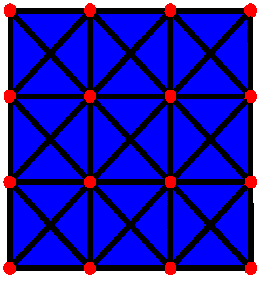
\includegraphics{report/figures/md_fisher_cloth.png}
    %\caption{Caption}
    %\label{fig:my_label}
%\end{figure}
%\todo{Find smaller image}

\subsection{What is Semi-Implicit Euler Integration?}
Semi-Implicit Euler integration is perhaps the integration scheme that is easiest to follow, and comes most natural to programmers when they implement
movement in a realtime system for the first time. \rephrase{It is also a scheme used within a lot of physics engines}\cite{gafferongames_integration}.
In Semi-Implicit Euler integration we keep the total accumulated force, velocity and position of each game object.
Upon each timestepped update of the system we divide all the force that has been applied to an object by the mass of the object to get the acceleration of the object.
Multiplying this acceleration with the timestep yields the change in velocity of the object, which added on the previous velocity becomes the new velocity.
This new velocity is then multiplied with the timestep and added to the position, reflecting the change in position over time.
The code for this can be seen in listing~\ref{code:semi-implicit_euler_integration}

\begin{figure}
\begin{lstlisting}[label={code:semi-implicit_euler_integration},language=csharp,caption={Semi-Implicit Euler Integration}]
private void SemiImplicitEuler(float dt, GameObject go)
{
    var acceleration = go.force / go.mass;
    go.velocity += acceleration * dt;
    go.position += go.velocity * dt;
}
\end{lstlisting}
\end{figure}

\subsubsection{Advantages \& Disadvantages}
The largest advantage of the Semi-Implicit Euler integration is its ease of implementation, as well as the generally low computational complexity.
However, it is not entirely stable, meaning that you can get into situations where your numbers start exploding.

\subsection{What is Verlet Integration?}
Rather than storing velocities and positions of each game object like the Euler integration, Verlet integration stores the current and previous positions of each game object.
Per timestep the current velocity is calculated implicitly by subtracting the current position from the previous one.
Changes to the current velocity is also modelled via positional data by integrating the game object's acceleration twice over the timestep.
The new position of a game object following a Verlet integration is then: The current position added with the calculated velocity and the positional change due to acceleration.
Code for this can be seen in listing~\ref{code:verlet_integration}.

\begin{figure}
\begin{lstlisting}[label={code:verlet_integration},language=csharp,caption={Verlet Integration}]
private void Verlet(float dt, GameObject go)
{
    var acceleration = go.force / go.mass;
    var curr = go.pos + (go.pos - go.prevPos) + acceleration * dt * dt;
    go.prevPos = go.pos;
    go.pos = curr;
}
\end{lstlisting}
\end{figure}

\subsubsection{Advantages \& Disadvantages}
Just like Semi-Implicit Euler integration this integration model is relatively easy to implement, and relatively fast.
Due to the velocity being calculated based on the positions, it is very hard to end up in a situation where the velocities and positions come out of sync,
meaning that the model is quite stable.
I would however argue that while it is easy to implement it is not as easy to understand as the Semi-Implicit Euler integration, at least upon first contact with the model.
I needed a proper intuitive explanation from Mosegaard\cite{mosegaards_clothing_simulation} before I understood what was really going on.

\subsection{Kinematic or Dynamic approach?}
When working with mesh deformation one needs to decide upon a kinematic or a dynamic approach.

Within a kinematic approach the springs between the vertices are thought of as constraints that you need to solve for.
I.e. if two points are two far apart from each other, you move them a bit closer together, potentially over several iterations to ensure that you are not creating
new inconsistencies in the model.
The kinematic approach is the easiest to implement of the two and can never explode, however, the extra iterations needed to solve the constraints can have performance implications.

The dynamic approach on the other hand models the springs as actual springs that correct themselves through force according to the laws of physics, such as Hooke's Law.
This approach is much harder to implement, and can lead to situations where the model spirals out of control (i.e. explodes).
Additionally, while implementing soft springs in with this approach is not that difficult, but harder springs require more complicated integration schemes\cite{math_for_games}.

While both of these approaches imply different terminology for the connections/springs within a system I will refer to the connections between vertices as springs for the rest of the article, as the name of the model is spring mass model.

\section{Dynamic Approach - Ball Deformation}
\todo{Add video}
Jasper Flick\cite{catlike_mesh_deformation} shows an implementation where the springs are implied based on the original position of each vertex and their new position.
The implementation takes a dynamic approach to deformation and follows a semi-implicit Euler integration scheme.
In this implementation we keep a copy of the initial vertex positions, as well as a collection of the modified vertices.
Additionally, we keep a collection of the velocity of each vertex, which we update each time force is added to a vertex.
The springs come into play when updating the positions of all the vertices based on their velocities.
Each spring within this system is the vector between the initial positions of the vertices in the mesh and their current positions, as seen in figure \ref{fig:catlike_mesh_deformation_springs}.
Upon update of the vertices the force of a spring is applied to the velocity of a vertex in the direction of the spring, moving the vertex back towards its initial position (see listing~\ref{code:catlike_mesh_deformation_update}).

\todo{Write about how force is added}

\begin{figure}
\centering
    \scalebox{0.5}{
    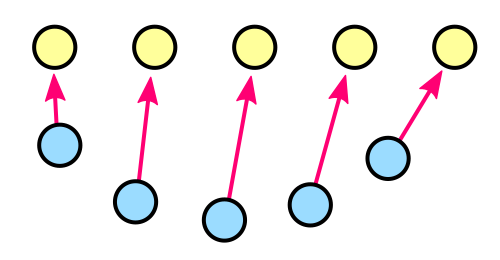
\includegraphics[width=\textwidth]{report/figures/catlike_mesh_deformation_springs.png}
    }
    \caption{Modified vertices(yellow) are pulled towards their original position(blue) by the springs (pink)\cite{catlike_mesh_deformation}}
    \label{fig:catlike_mesh_deformation_springs}
\end{figure}

\begin{figure}
\begin{lstlisting}[label={code:catlike_mesh_deformation_update},language=csharp,caption={Catlike coding mesh deformation vertex update}]
private void UpdateVertex(int i)
{
    Vector3 velocity = mVertexVelocities[i];
    Vector3 spring = mDisplacedVertices[i] - mOriginalVertices[i];
    spring *= UniformScale;
    velocity -= spring * SpringForce * Time.deltaTime;
    velocity *= 1f - Damping * Time.deltaTime;
    mVertexVelocities[i] = velocity;
    mDisplacedVertices[i] += velocity * (Time.deltaTime / UniformScale);
}
\end{lstlisting}
\end{figure}

\subsection{Usage}
As seen from the video, although simple, the implementation provides quite a lot of flexibility, toying with the different variables
can lead to some interesting visual effects.
For example, applying negative force to the sphere can be used to create a visual effect similar to that of a star being swallowed by a black hole.
Applying outward force from the inside of the model can create a relatively convincing effect of something moving around inside the object.
Giving the sphere a high SpringForce will lead to it being harder to deform, and more bouncy when trying to return to its original shape.

\subsection{Limitations}
As previously mentioned the implementation is quite simple, but has some limitations.
As mentioned by Flick\cite{catlike_mesh_deformation} this implementation is not a physics simulation, while the mesh is deformed
the colliders and physical representation of the object stays the same.
Additionally, none of the vertices are connected to each other through springs, and therefore move completely independent from each other.
This means that if we were to for instance pin two of the vertices to their initial position, and then apply force to the mesh
none of the other vertices would respect that two of them was locked in place, leading to less than satisfying results.

\section{Kinematic Approach - Cloth Simulation}
Cloth simulation is a place where the springs are more apparent than the previous implementation.
The implementation seen in Figure \ref{fig:my_cloth_implementation_springs} shows all the springs needed to create a believable cloth simulation.
The implementation is based on that of Jesper Mosegaard\cite{mosegaards_clothing_simulation} and Thomas Jakobsen\cite{jakobsen_advanced_character_physics}.
Unlike the previous implementation, the springs here are explicit and ensure that vertices are not handled in isolation but rather are affected by the other vertices in the system.
This gives greater control in that it allows you to apply force to a specific vertex and the whole system responds, rather than having to apply the force to all the vertices.

\begin{figure}
%\centering
%    \caption{\todo{Insert figure}}
    \label{fig:my_cloth_implementation_springs}
\end{figure}

\subsection{Spring Types}
There are three types of springs within this implementation, all serving the same purpose of holding the model together,
but in different ways. The different types can be seen in figure~\ref{fig:spring_types}
\begin{figure}
    \centering
    \caption{The different spring types (here labeled constraints). Image taken from Jesper Mosegaard\cite{mosegaards_clothing_simulation}}
    \scalebox{0.5}{
    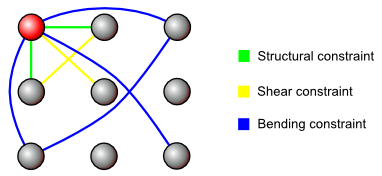
\includegraphics[width=\textwidth]{report/figures/spring_types.png}
    }
    \label{fig:spring_types}
\end{figure}

\subsubsection{Structural Springs}
The structural springs are the vertical and horizontal connections between the vertices,
ensure that the model stays in one piece.
However, they alone are not enough, as the model can collapse into itself in a two dimensional space\cite{jeff_lander_real_time_cloth} this can be seen in figure~\ref{fig:structural_springs_collapsing}.

\begin{figure}[H]
    \centering
    \caption{Cloth of only structural springs in the process of collapsing into itself}
    \scalebox{0.5}{
    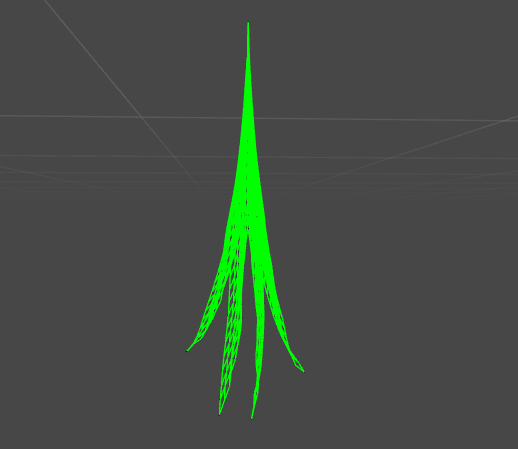
\includegraphics[width=\textwidth]{report/figures/structural_collapse.png}
    }
    \label{fig:structural_springs_collapsing}
\end{figure}

\subsubsection{Shear Springs}
Shear springs fixes the issue mentioned above by a connection between each vertex and their diagonal members.
When the vertices are about to start collapsing in on themselves the shear springs will push them apart again\cite{jeff_lander_real_time_cloth}.
These springs also helps the model to act in a three dimensional space.
Since the vertices no longer can collapse in on themselves they might need to make use of three dimensions to
resolve their collisions, as seen in figure~\ref{fig:shear_springs_collapsing}.
\begin{figure}[H]
    \centering
    \caption{Cloth of structural and shear springs, preventing it from collapsing into 2D space}
    \scalebox{0.5}{
    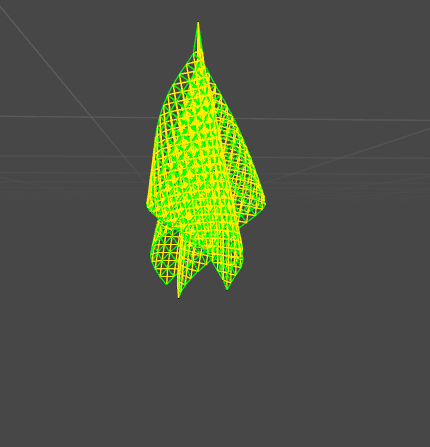
\includegraphics[width=\textwidth]{report/figures/shear_collapse.png}
    }
    \label{fig:shear_springs_collapsing}
\end{figure}

\subsubsection{Bending Springs}
Technically you only need these two types of springs to create an ok looking cloth simulation,
however a third type of spring called bending springs can be added.
These are connected between each vertex and their second neighbour,
which can help fix cases where the second neighbour of a vertex is unrealistically placed in the system.
This in general leads to the cloth becoming more flat, as extreme differences between the vertices are corrected for
through the second neighbouring vertices\cite{jeff_lander_real_time_cloth}.
While not as obvious, this can be seen in figure~\ref{fig:bending_springs_collapsing}.
\begin{figure}[H]
    \centering
    \caption{Cloth of structural, shear, and bending strings, preventing it from bending unrealistically into itself.}
    \scalebox{0.5}{
    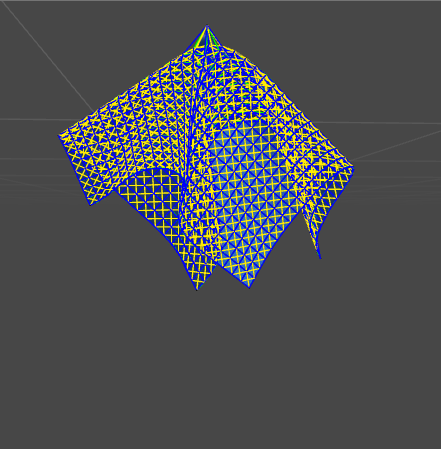
\includegraphics[width=\textwidth]{report/figures/bending_collapse.png}
    }
    \label{fig:bending_springs_collapsing}
\end{figure}

\todo{Mention that all the springs have the same force, that might be something we want to change}

% This might be what is creating wrinkles?
% Double check that this is actually the case.
% Without
%
% 1 -- 2
%      |
%      3
% With
% ------------|
% 1 -- 2 ---| |
%           3 -

\subsection{Implementation}
In this implementation we keep all the springs within a collection, each spring knowing which two vertices they are connected to and the desired rest length of the spring.
Upon update we iterate through all the vertices and calculate their new positions based on the Verlet integration scheme.
Following the update is fixing the constraints. This is done by iterating through all the springs and correcting the distance between the vertices it is connected to.
This needs to be done several times as to avoid the model seeming to elastic.
The code for this can be seen in listing~\ref{code:satisfy_constraints}.


\begin{figure}
\begin{lstlisting}[label={code:satisfy_constraints},language=csharp,caption={Semi-Implicit Euler Integration}]
private void FixedUpdate()
{
    for (int step = 0; step < ConstraintIterations; step++)
    {
        for (int i = 0; i < mSprings.Count; i++)
        {
            var spring = mSprings[i];
            var diff = mPositions[spring.V2Idx] - mPositions[spring.V1Idx];
            var dist = diff.magnitude;
            var correction = (diff * (1 - spring.RestDistance / dist)) * 0.5f;

            mPositions[spring.V1Idx] += correction;
            mPositions[spring.V2Idx] -= correction;
        }
    }
}
\end{lstlisting}
\end{figure}

\subsection{Usage}
Due to its more sophisticated nature this implementation offers more flexibility than the previous one.
Simulation of entire pieces of clothes like curtains or flags are obvious ways of using this model.
However, it is not a requirement of the model that every vertex in a mesh are simulated and part of the mass spring system, you can also just simulate parts of it.
An example here is if you have a character wearing a dress, you probably do not need that every part of the dress
has realistic cloth physics, it is probably enough that just the bottom of the dress reacts to the environment
to create a believable appearance.
\todo{Add image showing parts of the model being simulated, as I don't think it is entirely clear from the text}

Another use case with this model could be to have cloth that tears at a certain point because it is stretched too much,
or that parts of the cloth is cut off. This should not be too difficult, you would need to remove the springs between
the vertices that have been disconnected from the rest of the model.
Additionally, you would have to ensure that all the cuts were in line with the triangles of the mesh.

\subsection{Issues}
Although there are many advantages of this model, like how it is relatively easy to implement, gives quite good results and cannot "explode", it does suffer from a few issues.
A problem with this implementation is that it can get into unsolvable states.
I.e. when you apply forces to model continuously it can get into a situation where it never rests.
Such a situation can be seen in the following video \todo{Add video}.
Here the forces of gravity are continuously being applied to the vertices, in the real world the bottom
of this cloth would stop moving after a while. However, in this implementation the cloth never stops moving
because the springs never manage to get into a situation where they all are "satisfied".
This is due to the kinematic approach chosen\cite{math_for_games}
The number of times you need to iterate over the constraints to satisfy them is also an issue.
Too few iterations and the cloth will look too elastic, too many iterations and it can seem too hard,
additionally, the more iterations you add, the more processing time is needed, which can become a performance problem.

\subsection{Extensions}
Matthew Fisher\cite{matthew_fisher} suggests some extensions to the model,
such as quilting. Currently the cloth looks like infinitely thin silk, which is not particularly realistic,
quilting would add thickness to the model, allowing it to look and act more like wool or cotton. 
Fisher suggests doing this with a marching cubes algorithm.
However, that would potentially be more costly to simulate and to draw.
Another extension could be self collision or collision with other soft bodies, however, this is very challenging to implement
and quickly ends up being really expensive in terms of performance as well.
Another extension would be to move these calculations over to the GPU, as a lot of the calculations that are done are data parallel,
and would therefore benefit from being executed in a parallel environment.

\todo{Bring up how an extension is to do this on a gpu}

\todo{Should I also look into the Catlike Coding water deformation thingy, as it is another way of doing mesh deformation}


\todo{The technology ahead, ask if this could be used with tesselation and be done on the GPU?}
\todo{Discuss how mass spring damper model also used for other stuff, such as water simulation. Look at Just Cause water implementation article on gamasutra}

\chapter{Users}
While cloth simulation and simple deformation effects are obvious usages of the spring mass system, it 

\chapter{Future}
Predicting the future is always a difficult challenge, especially in fields such as technology and graphics.
However, I would say that it seems like we have settled down on some of the classic conceptual techniques such as spring mass systems, finite element methods and meshless deformations~\cite{muller2005meshless}, at least for interactive applications such as video games. 

I base this on how the mass spring model, although quite old, is still brought in many of the slides I have seen on cloth simulation from different universities such as Trinity College in Dublin\cite{mass_spring_cloth_trinity},
and its continuous use in the games industry.
For example the clothing in Alan Wake\footnote{\url{http://www.alanwake.com/}} was done through a mass spring model\cite{alan_wake_mass_spring}, and from my impression this is also the case
in Assassin's Creed Unity\footnote{\url{https://www.ubisoft.com/en-us/game/assassins-creed-unity/}} and Far Cry 4\footnote{\url{https://www.ubisoft.com/en-us/game/far-cry-4/}}\cite{ubisoft_cloth_simulation}.
This might change in the future though as other models are proposed. Weidner et al.~\cite{weidner_eol} proposes a way to deal with the situation where a piece of cloth collides with a straight edges that are not exactly on the vertices leading to sub-realistic results. 
However, it is not entirely clear to me how this implementation actually works and whether or not it is for real-time applications such as games, or would require too much processing power. 
If that is the case, maybe it will be possible in the future.

While other methods do exist I do not think we will move away from spring mass systems very soon, their relative easy of implementation, believably,
and relatively good performance still make them attractive.
It is important to remember that it is not always about having the newest shiniest tool, but rather using that tool that best fit the situation at hand.


\todo{Bring up that the methods today might be enough, i.e. we don't really need more, it's not the same ompf factor, and today is satisfying}

\think{Conclussion:
Spring mass systems even in their most basic forms will still probably stick around,
as it is a reasonably simple and not to taxing approach that gives plausible results.
}

%\todo{Hybrid Systems?, (D4MD – Deformation system for a vehicle simulation game) }
%* Eulerian-on-langrangian cloth simulation: \url{https://drive.google.com/file/d/1l3zUKHi1TVbmF_SweB6FB3xCa5XBQ6mF/view}
%* Nonsmooth Developable Geometry for Interactively Animating Paper Crumpling: \url{https://dl.acm.org/citation.cfm?doid=2870647.2829948}

% http://www.gamasutra.com/view/feature/132771/the_secrets_of_cloth_simulation_in_.php?page=4
\chapter{Sources}
\chapter{Reflection}
Working on this project has been an enlightening experience, but it has not been without issues.
Originally I wanted to look at shaders in Unity to brush up on my shader knowledge, with the final goal being to end up in the area of terrain deformation.
I spent the beginning of the project toying with Unity's shadergraph\footnote{\url{https://blogs.unity3d.com/2018/02/27/introduction-to-shader-graph-build-your-shaders-with-a-visual-editor/}}, creating different visual effects\footnote{\todo{Add video of the simple shielding effect}} to verify that my assumptions of how shaders actually worked were correct. 

After getting my feet wet in shadergraph I moved over to writing the shaders by hand, while looking for tutorials on terrain deformation.
It was hard to find good tutorials on this, especially on the GPU. However, I did stumble across a seemingly good tutorial from Jasper Flick\footnote{\url{https://catlikecoding.com/unity/tutorials/advanced-rendering/surface-displacement/}} 
on surface displacement which seemed quite close to what I wanted to do.
This tutorial assumed that you were already quite familiar with rendering concepts, and built on his previous tutorials, so I started going through those.
While working through these tutorials I felt that Unity's shaders were too different from those I had written before in OpenGL, the learning curve
was a bit too steep, debugging tools were quite lacking, and that I was not making good progress towards the end goal.

I looked around for alternative solutions. Writing shaders in Unreal was a possibility, but that requires building the entire engine from source
when you add your own shading models\cite{unreal_shaders}, and the compilation times would quickly hurt my iteration process.
Another alternative was to implement my own rendering program in C++, but that would have taken too much time.

Due to this I decided to move back to the CPU, and work on more general mesh deformation there.
The original intention was to port the logic over to vertex shaders after I had implemented them on the CPU.
I soon moved away from that idea. Implementing stuff on the GPU probably would be more of a chore than a learning experience,
as I already have dealt with data layout and CPU-GPU communication in other courses.
The challenge would be the logic of mesh deformation, not how to do it in shaders.

With the shift over to the CPU I started to work on procedural mesh generation, as all the different tutorials I looked at
on mesh deformation was working on procedurally generated meshes. Working through the procedural mesh generation tutorials
of Jasper Flick was quite intuitive and gave results, and in the end I finished his mesh deformation tutorial.
I played around with the implementation for a while, without a clear goal of where to next.

Looking through papers on the topic of mesh deformation most of it seemed to focus on deformation for manipulating meshes more related to creating animations,
which was not really what I was after. 
It was first when I learned that the mesh deformation that Jasper Flick\cite{catlike_mesh_deformation} presented was a sort of mass spring system
that I figured out that deformation through mass spring systems would be what I wanted to focus on, and its use in cloth simulation was quite enticing.
Unfortunately, this was quite late in the course, so I did not get to spend as much time on the background of the technology, alternatives
and the future of the technology as I originally wanted.
I would have loved to get more into the other approaches like the finite element methods or free form deformations, or try the mass spring system
within other contexts or with other integrators, moving more into the area of physics simulations.
Figuring out the topic so late also meant that I ran into the problem that you do not really know what to search for until you have been in an area for a while,
which meant that looking around for more background papers and tutorials was quite difficult.

However, while the path I took throughout this project was full of twists and turns I do believe I have come out of it with a greater and wider understanding of
shaders \& rendering, mesh manipulation, and physically based deformation.



% * Wanted to look at terrain deformation like that seen in god of war, though it would all be done in shaders
% * Generalized this Unity shaders (as I wanted to get back into shaders coding, toyed with shadergraph and shaders for a bit, doing tutorials)
%     * Worked towards Surface displacement in catlike coding
%     * Unity Shaders was way to different than the OpenGL shaders I was used to
%         * Tried moving over to Unreal, but apparently had to compile from source to get proper shader support
%             * Compilation times would kill my iteration times.
%             * Writing my own implementation would take too much time.
%     * Move over to mesh deformation on the CPU first
%         * The convert to the GPU
%         * Doing stuff on the GPU is a bit harder, but after having implemented it on the CPU, implementing it on the GPU is more of a chore
%             * Figuring out data layout etc, I have already done that a lot before, so re-implementing stuff on the GPU will probably be more of a chore with poor debugging tools,
%                 rather than a task I really learn something new from.
%     * Move over to only doing it on the CPU, still with target to do terrain deformation
% * Worked towards the mesh deformation shown on catlike coding
%     * Didn't really find any good tutorials on terrain deformation in specific.
%     * After implementing it, learned that it was called spring mass systems
%     * Got more interested in the system and deformations in general, saw that the system could be used for cloth simulation.
%     * Moved over to doing cloth physics.
% * The road to the end has been full of twists and turns, however, I believe I have come out of it with a greater and wider understanding of both shaders, and mesh manipulation,
% although the shaders are not really reflected in the end product.
    
    



%\chapter{Structural Elements}
\label{chap:structural}

If you are submitting using the DAIM system you should make sure the pdf you submit does not have the front page information, as that will be added by the submission form in DAIM.  You can remove the DAIM option to print the front page material if you want a full PDF with the front page material. To make sure the running header has the title of the thesis you still need to set it in the \verb+DaimData.tex+ file. The title of the thesis should be set using the \verb+\thesistitle+
command, and the date of the thesis should be set using the
\verb+\thesisdate+ command in the \verb+DaimData.tex+ file. 

\section{Page Layout}

The geometry of the page has been set using the \verb+\geometry+
command.

\section{Fonts}

Due to limited \LaTeX\ support for the Georgia font, Charter has been
chosen instead. For mathematical formula, the Euler fonts are used,
since they blend more nicely with the Charter than the standard
\LaTeX\ fonts: 
\begin{equation} \label{eq:1}
    f(x) = \int_0^x g(\tau)\,d\tau
\end{equation}



For inline math you can use $\backslash{}($ and $\backslash{})$ for example \( f(x)= \frac{x^2}{1+x^2} \).  
This also allows you to use $\slash$ and $\backslash$. You need to include the \{\} when you want the special
character to have other letters immediately after it.

\section{Sectioning Commands}

The standard \LaTeX\ sectioning commands are used for both numbered
and unnumbered sections. The top level is given by the \verb+\chapter+
command. This starts a new right page. The two lower levels are
obtained using the \verb+\section+ and \verb+\subsection+ commands.
The standard \LaTeX\ \verb+\subsubsection+ and \verb+\paragraph+
commands have been disabled since their use is not encouraged by the
thesis guidelines. When you use these they will not be given numbers.  
They still appear in the document with highlighting but not in the 
table of contents.

\subsection{The subsection}

This is an example of a subsection.

\subsubsection{The subsubsection}

This is an example of a subsubsection.

\paragraph{The paragraph}

This is an example of a paragraph with a heading.

\section{Floats (Figures and Tables)}
\label{sec:floats}

Figures are placed in the \texttt{figure} environment. An example is
shown in Figure~\ref{fig:example}. %notice the ~ in between figure and the \ref. it stops latex from splitting the number and word over a line.
Tables are placed in the \texttt{table} environment. An example is given in
Table~\ref{tab:example} and reading the information directly from file in Table~\ref{tab:examplecsv}. Figures and tables float freely around in the
document in accordance with standard \LaTeX\ behavior.

\begin{figure}[tbp]  %t top, b bottom, p page | you can also use h to try to get the figure to appear at the current location
  \centering
  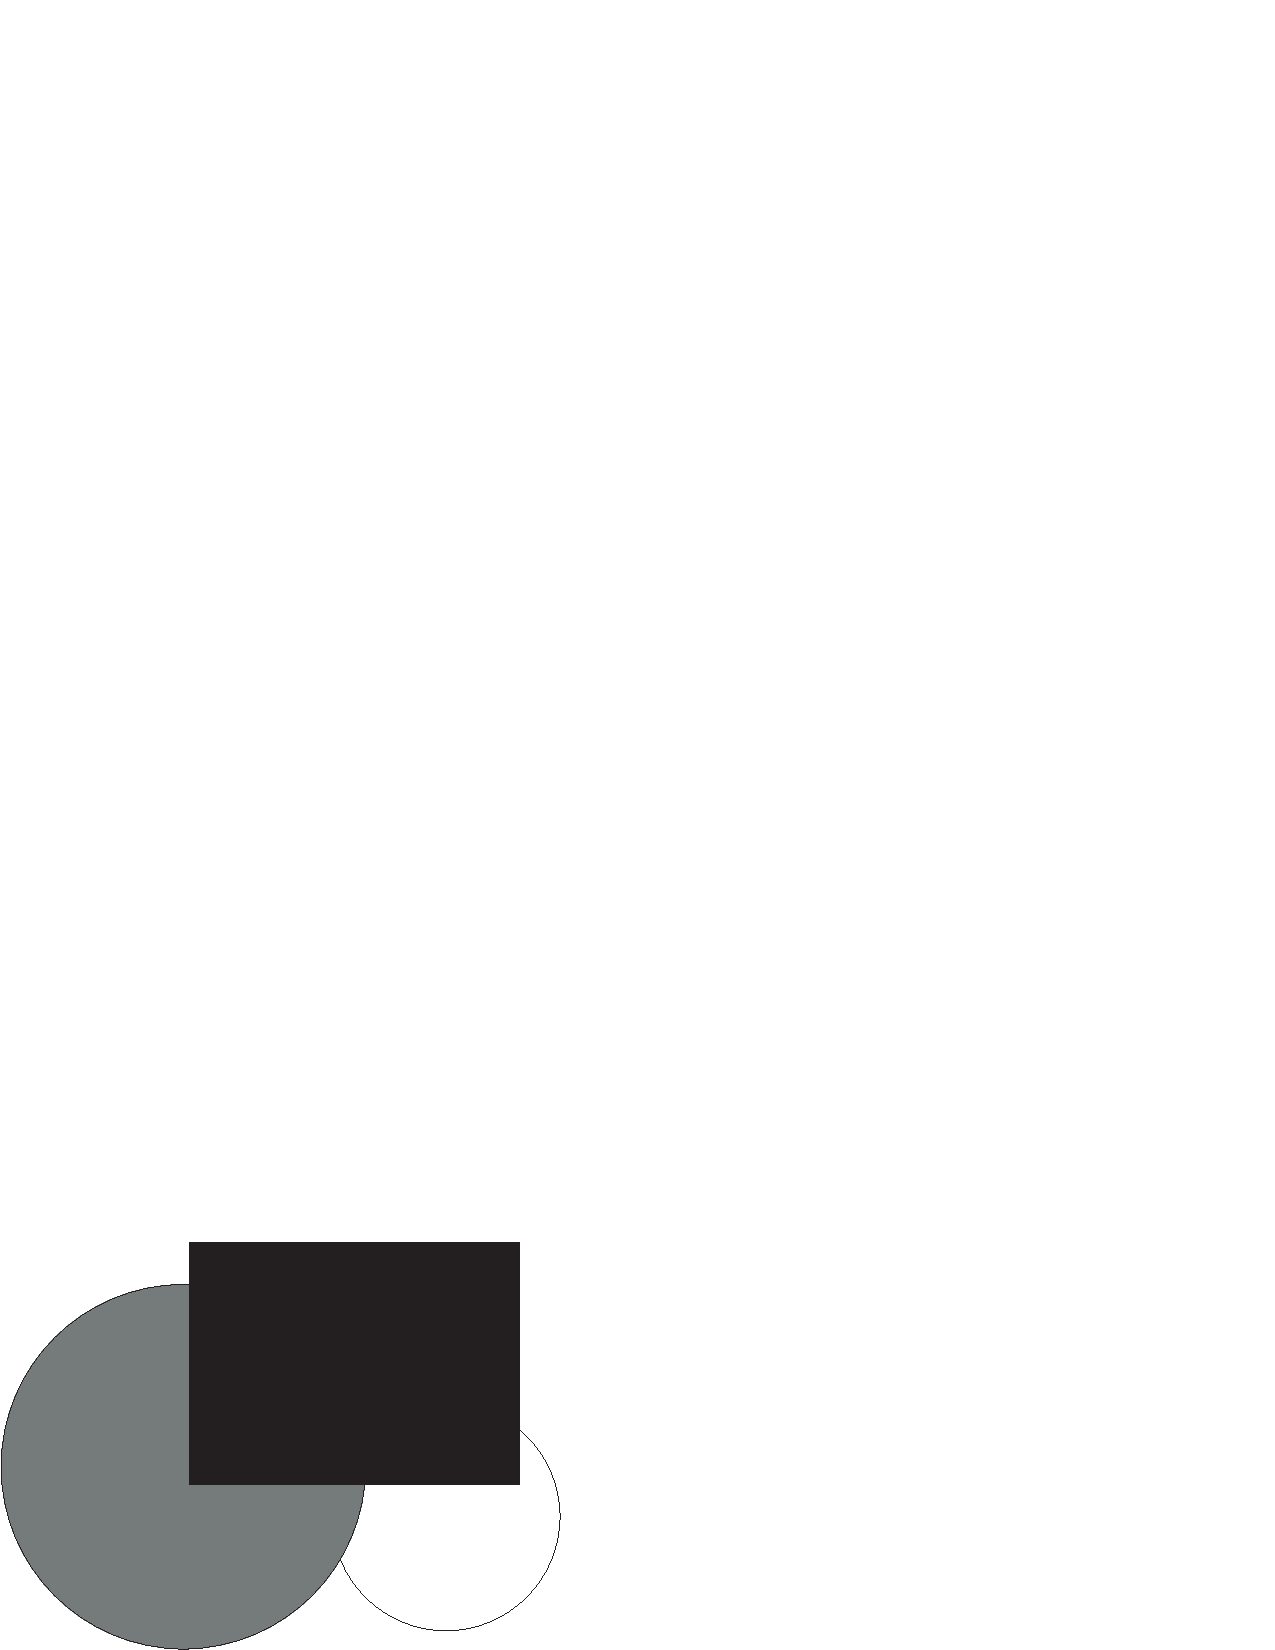
\includegraphics[width=.5\textwidth]{figures/example_fig}
  \caption[An example figure.]{An example figure. If the caption is
    shorter than one line, it is centered. If it goes over more than
    one line, it is left and right justified. Furthermore, it is
    suggested that an alternative short caption is given in order to
    produce a good list of figures.}
  \label{fig:example}
\end{figure}

\begin{table}[tbp]
  \centering
  \begin{tabular}{c|c}
    Age  & IQ  \\ 
    \hline
    10   & 100 \\
    20   & 100 \\
    30   & 150 \\
    40   & 100 \\
    50   & 100
  \end{tabular}
  \caption{An example table.}
  \label{tab:example}
\end{table}

\begin{table}[tbp]
  \centering
  \csvautobooktabular{figures/ageiq.csv}
  \caption{An example table using simplecsv.}
  \label{tab:examplecsv}
\end{table}

The captions are placed \emph{below} both for the figures and the
tables. The caption is set in 9pt. If the caption is shorter than one
line, it is centered.

\subsection{Gnuplot}
There are many ways to include graphs in your document.  Figure~\ref{fig:exgnuplotex} for including a file generated by gnuplot and saved as \texttt{gnuplotgraph1.tex}. 
%Figure~\ref{fig:exgnuplotintegrate} shows how to include the script to generate a graph direction in \LaTeX.

\begin{figure}[htp]  %t top, b bottom, p page | you can also use h to try to get the figure to appear at the current location
  \centering
  % GNUPLOT: LaTeX picture
\setlength{\unitlength}{0.240900pt}
\ifx\plotpoint\undefined\newsavebox{\plotpoint}\fi
\begin{picture}(1500,900)(0,0)
\sbox{\plotpoint}{\rule[-0.200pt]{0.400pt}{0.400pt}}%
\put(130.0,82.0){\rule[-0.200pt]{4.818pt}{0.400pt}}
\put(110,82){\makebox(0,0)[r]{-1}}
\put(1419.0,82.0){\rule[-0.200pt]{4.818pt}{0.400pt}}
\put(130.0,151.0){\rule[-0.200pt]{4.818pt}{0.400pt}}
\put(110,151){\makebox(0,0)[r]{-0.8}}
\put(1419.0,151.0){\rule[-0.200pt]{4.818pt}{0.400pt}}
\put(130.0,221.0){\rule[-0.200pt]{4.818pt}{0.400pt}}
\put(110,221){\makebox(0,0)[r]{-0.6}}
\put(1419.0,221.0){\rule[-0.200pt]{4.818pt}{0.400pt}}
\put(130.0,290.0){\rule[-0.200pt]{4.818pt}{0.400pt}}
\put(110,290){\makebox(0,0)[r]{-0.4}}
\put(1419.0,290.0){\rule[-0.200pt]{4.818pt}{0.400pt}}
\put(130.0,360.0){\rule[-0.200pt]{4.818pt}{0.400pt}}
\put(110,360){\makebox(0,0)[r]{-0.2}}
\put(1419.0,360.0){\rule[-0.200pt]{4.818pt}{0.400pt}}
\put(130.0,429.0){\rule[-0.200pt]{4.818pt}{0.400pt}}
\put(110,429){\makebox(0,0)[r]{ 0}}
\put(1419.0,429.0){\rule[-0.200pt]{4.818pt}{0.400pt}}
\put(130.0,498.0){\rule[-0.200pt]{4.818pt}{0.400pt}}
\put(110,498){\makebox(0,0)[r]{ 0.2}}
\put(1419.0,498.0){\rule[-0.200pt]{4.818pt}{0.400pt}}
\put(130.0,568.0){\rule[-0.200pt]{4.818pt}{0.400pt}}
\put(110,568){\makebox(0,0)[r]{ 0.4}}
\put(1419.0,568.0){\rule[-0.200pt]{4.818pt}{0.400pt}}
\put(130.0,637.0){\rule[-0.200pt]{4.818pt}{0.400pt}}
\put(110,637){\makebox(0,0)[r]{ 0.6}}
\put(1419.0,637.0){\rule[-0.200pt]{4.818pt}{0.400pt}}
\put(130.0,707.0){\rule[-0.200pt]{4.818pt}{0.400pt}}
\put(110,707){\makebox(0,0)[r]{ 0.8}}
\put(1419.0,707.0){\rule[-0.200pt]{4.818pt}{0.400pt}}
\put(130.0,776.0){\rule[-0.200pt]{4.818pt}{0.400pt}}
\put(110,776){\makebox(0,0)[r]{ 1}}
\put(1419.0,776.0){\rule[-0.200pt]{4.818pt}{0.400pt}}
\put(130.0,82.0){\rule[-0.200pt]{0.400pt}{4.818pt}}
\put(130,41){\makebox(0,0){-10}}
\put(130.0,756.0){\rule[-0.200pt]{0.400pt}{4.818pt}}
\put(457.0,82.0){\rule[-0.200pt]{0.400pt}{4.818pt}}
\put(457,41){\makebox(0,0){-5}}
\put(457.0,756.0){\rule[-0.200pt]{0.400pt}{4.818pt}}
\put(785.0,82.0){\rule[-0.200pt]{0.400pt}{4.818pt}}
\put(785,41){\makebox(0,0){ 0}}
\put(785.0,756.0){\rule[-0.200pt]{0.400pt}{4.818pt}}
\put(1112.0,82.0){\rule[-0.200pt]{0.400pt}{4.818pt}}
\put(1112,41){\makebox(0,0){ 5}}
\put(1112.0,756.0){\rule[-0.200pt]{0.400pt}{4.818pt}}
\put(1439.0,82.0){\rule[-0.200pt]{0.400pt}{4.818pt}}
\put(1439,41){\makebox(0,0){ 10}}
\put(1439.0,756.0){\rule[-0.200pt]{0.400pt}{4.818pt}}
\put(130.0,82.0){\rule[-0.200pt]{0.400pt}{167.185pt}}
\put(130.0,82.0){\rule[-0.200pt]{315.338pt}{0.400pt}}
\put(1439.0,82.0){\rule[-0.200pt]{0.400pt}{167.185pt}}
\put(130.0,776.0){\rule[-0.200pt]{315.338pt}{0.400pt}}
\put(784,838){\makebox(0,0){Test of $y=sin(x)$}}
\put(785,429){\makebox(0,0)[l]{$y=sin(x)$}}
\put(1279,736){\makebox(0,0)[r]{sin(x)}}
\put(1299.0,736.0){\rule[-0.200pt]{24.090pt}{0.400pt}}
\put(130,618){\usebox{\plotpoint}}
\multiput(130.58,609.67)(0.493,-2.439){23}{\rule{0.119pt}{2.008pt}}
\multiput(129.17,613.83)(13.000,-57.833){2}{\rule{0.400pt}{1.004pt}}
\multiput(143.58,546.90)(0.493,-2.677){23}{\rule{0.119pt}{2.192pt}}
\multiput(142.17,551.45)(13.000,-63.450){2}{\rule{0.400pt}{1.096pt}}
\multiput(156.58,479.28)(0.494,-2.553){25}{\rule{0.119pt}{2.100pt}}
\multiput(155.17,483.64)(14.000,-65.641){2}{\rule{0.400pt}{1.050pt}}
\multiput(170.58,408.77)(0.493,-2.717){23}{\rule{0.119pt}{2.223pt}}
\multiput(169.17,413.39)(13.000,-64.386){2}{\rule{0.400pt}{1.112pt}}
\multiput(183.58,340.15)(0.493,-2.598){23}{\rule{0.119pt}{2.131pt}}
\multiput(182.17,344.58)(13.000,-61.577){2}{\rule{0.400pt}{1.065pt}}
\multiput(196.58,274.92)(0.493,-2.360){23}{\rule{0.119pt}{1.946pt}}
\multiput(195.17,278.96)(13.000,-55.961){2}{\rule{0.400pt}{0.973pt}}
\multiput(209.58,216.42)(0.494,-1.892){25}{\rule{0.119pt}{1.586pt}}
\multiput(208.17,219.71)(14.000,-48.709){2}{\rule{0.400pt}{0.793pt}}
\multiput(223.58,165.35)(0.493,-1.607){23}{\rule{0.119pt}{1.362pt}}
\multiput(222.17,168.17)(13.000,-38.174){2}{\rule{0.400pt}{0.681pt}}
\multiput(236.58,125.75)(0.493,-1.171){23}{\rule{0.119pt}{1.023pt}}
\multiput(235.17,127.88)(13.000,-27.877){2}{\rule{0.400pt}{0.512pt}}
\multiput(249.58,97.67)(0.493,-0.576){23}{\rule{0.119pt}{0.562pt}}
\multiput(248.17,98.83)(13.000,-13.834){2}{\rule{0.400pt}{0.281pt}}
\put(262,83.17){\rule{2.700pt}{0.400pt}}
\multiput(262.00,84.17)(7.396,-2.000){2}{\rule{1.350pt}{0.400pt}}
\multiput(275.00,83.58)(0.582,0.492){21}{\rule{0.567pt}{0.119pt}}
\multiput(275.00,82.17)(12.824,12.000){2}{\rule{0.283pt}{0.400pt}}
\multiput(289.58,95.00)(0.493,1.012){23}{\rule{0.119pt}{0.900pt}}
\multiput(288.17,95.00)(13.000,24.132){2}{\rule{0.400pt}{0.450pt}}
\multiput(302.58,121.00)(0.493,1.527){23}{\rule{0.119pt}{1.300pt}}
\multiput(301.17,121.00)(13.000,36.302){2}{\rule{0.400pt}{0.650pt}}
\multiput(315.58,160.00)(0.493,1.924){23}{\rule{0.119pt}{1.608pt}}
\multiput(314.17,160.00)(13.000,45.663){2}{\rule{0.400pt}{0.804pt}}
\multiput(328.58,209.00)(0.494,2.113){25}{\rule{0.119pt}{1.757pt}}
\multiput(327.17,209.00)(14.000,54.353){2}{\rule{0.400pt}{0.879pt}}
\multiput(342.58,267.00)(0.493,2.558){23}{\rule{0.119pt}{2.100pt}}
\multiput(341.17,267.00)(13.000,60.641){2}{\rule{0.400pt}{1.050pt}}
\multiput(355.58,332.00)(0.493,2.717){23}{\rule{0.119pt}{2.223pt}}
\multiput(354.17,332.00)(13.000,64.386){2}{\rule{0.400pt}{1.112pt}}
\multiput(368.58,401.00)(0.493,2.757){23}{\rule{0.119pt}{2.254pt}}
\multiput(367.17,401.00)(13.000,65.322){2}{\rule{0.400pt}{1.127pt}}
\multiput(381.58,471.00)(0.493,2.677){23}{\rule{0.119pt}{2.192pt}}
\multiput(380.17,471.00)(13.000,63.450){2}{\rule{0.400pt}{1.096pt}}
\multiput(394.58,539.00)(0.494,2.333){25}{\rule{0.119pt}{1.929pt}}
\multiput(393.17,539.00)(14.000,59.997){2}{\rule{0.400pt}{0.964pt}}
\multiput(408.58,603.00)(0.493,2.241){23}{\rule{0.119pt}{1.854pt}}
\multiput(407.17,603.00)(13.000,53.152){2}{\rule{0.400pt}{0.927pt}}
\multiput(421.58,660.00)(0.493,1.845){23}{\rule{0.119pt}{1.546pt}}
\multiput(420.17,660.00)(13.000,43.791){2}{\rule{0.400pt}{0.773pt}}
\multiput(434.58,707.00)(0.493,1.408){23}{\rule{0.119pt}{1.208pt}}
\multiput(433.17,707.00)(13.000,33.493){2}{\rule{0.400pt}{0.604pt}}
\multiput(447.58,743.00)(0.494,0.827){25}{\rule{0.119pt}{0.757pt}}
\multiput(446.17,743.00)(14.000,21.429){2}{\rule{0.400pt}{0.379pt}}
\multiput(461.00,766.58)(0.652,0.491){17}{\rule{0.620pt}{0.118pt}}
\multiput(461.00,765.17)(11.713,10.000){2}{\rule{0.310pt}{0.400pt}}
\multiput(474.00,774.93)(1.378,-0.477){7}{\rule{1.140pt}{0.115pt}}
\multiput(474.00,775.17)(10.634,-5.000){2}{\rule{0.570pt}{0.400pt}}
\multiput(487.58,768.29)(0.493,-0.695){23}{\rule{0.119pt}{0.654pt}}
\multiput(486.17,769.64)(13.000,-16.643){2}{\rule{0.400pt}{0.327pt}}
\multiput(500.58,748.50)(0.493,-1.250){23}{\rule{0.119pt}{1.085pt}}
\multiput(499.17,750.75)(13.000,-29.749){2}{\rule{0.400pt}{0.542pt}}
\multiput(513.58,715.37)(0.494,-1.599){25}{\rule{0.119pt}{1.357pt}}
\multiput(512.17,718.18)(14.000,-41.183){2}{\rule{0.400pt}{0.679pt}}
\multiput(527.58,669.82)(0.493,-2.083){23}{\rule{0.119pt}{1.731pt}}
\multiput(526.17,673.41)(13.000,-49.408){2}{\rule{0.400pt}{0.865pt}}
\multiput(540.58,615.67)(0.493,-2.439){23}{\rule{0.119pt}{2.008pt}}
\multiput(539.17,619.83)(13.000,-57.833){2}{\rule{0.400pt}{1.004pt}}
\multiput(553.58,553.03)(0.493,-2.638){23}{\rule{0.119pt}{2.162pt}}
\multiput(552.17,557.51)(13.000,-62.514){2}{\rule{0.400pt}{1.081pt}}
\multiput(566.58,486.28)(0.494,-2.553){25}{\rule{0.119pt}{2.100pt}}
\multiput(565.17,490.64)(14.000,-65.641){2}{\rule{0.400pt}{1.050pt}}
\multiput(580.58,415.77)(0.493,-2.717){23}{\rule{0.119pt}{2.223pt}}
\multiput(579.17,420.39)(13.000,-64.386){2}{\rule{0.400pt}{1.112pt}}
\multiput(593.58,347.03)(0.493,-2.638){23}{\rule{0.119pt}{2.162pt}}
\multiput(592.17,351.51)(13.000,-62.514){2}{\rule{0.400pt}{1.081pt}}
\multiput(606.58,280.79)(0.493,-2.400){23}{\rule{0.119pt}{1.977pt}}
\multiput(605.17,284.90)(13.000,-56.897){2}{\rule{0.400pt}{0.988pt}}
\multiput(619.58,220.94)(0.493,-2.043){23}{\rule{0.119pt}{1.700pt}}
\multiput(618.17,224.47)(13.000,-48.472){2}{\rule{0.400pt}{0.850pt}}
\multiput(632.58,170.48)(0.494,-1.562){25}{\rule{0.119pt}{1.329pt}}
\multiput(631.17,173.24)(14.000,-40.242){2}{\rule{0.400pt}{0.664pt}}
\multiput(646.58,128.75)(0.493,-1.171){23}{\rule{0.119pt}{1.023pt}}
\multiput(645.17,130.88)(13.000,-27.877){2}{\rule{0.400pt}{0.512pt}}
\multiput(659.58,100.41)(0.493,-0.655){23}{\rule{0.119pt}{0.623pt}}
\multiput(658.17,101.71)(13.000,-15.707){2}{\rule{0.400pt}{0.312pt}}
\multiput(672.00,84.95)(2.695,-0.447){3}{\rule{1.833pt}{0.108pt}}
\multiput(672.00,85.17)(9.195,-3.000){2}{\rule{0.917pt}{0.400pt}}
\multiput(685.00,83.58)(0.704,0.491){17}{\rule{0.660pt}{0.118pt}}
\multiput(685.00,82.17)(12.630,10.000){2}{\rule{0.330pt}{0.400pt}}
\multiput(699.58,93.00)(0.493,0.972){23}{\rule{0.119pt}{0.869pt}}
\multiput(698.17,93.00)(13.000,23.196){2}{\rule{0.400pt}{0.435pt}}
\multiput(712.58,118.00)(0.493,1.448){23}{\rule{0.119pt}{1.238pt}}
\multiput(711.17,118.00)(13.000,34.430){2}{\rule{0.400pt}{0.619pt}}
\multiput(725.58,155.00)(0.493,1.924){23}{\rule{0.119pt}{1.608pt}}
\multiput(724.17,155.00)(13.000,45.663){2}{\rule{0.400pt}{0.804pt}}
\multiput(738.58,204.00)(0.493,2.241){23}{\rule{0.119pt}{1.854pt}}
\multiput(737.17,204.00)(13.000,53.152){2}{\rule{0.400pt}{0.927pt}}
\multiput(751.58,261.00)(0.494,2.333){25}{\rule{0.119pt}{1.929pt}}
\multiput(750.17,261.00)(14.000,59.997){2}{\rule{0.400pt}{0.964pt}}
\multiput(765.58,325.00)(0.493,2.717){23}{\rule{0.119pt}{2.223pt}}
\multiput(764.17,325.00)(13.000,64.386){2}{\rule{0.400pt}{1.112pt}}
\multiput(778.58,394.00)(0.493,2.757){23}{\rule{0.119pt}{2.254pt}}
\multiput(777.17,394.00)(13.000,65.322){2}{\rule{0.400pt}{1.127pt}}
\multiput(791.58,464.00)(0.493,2.717){23}{\rule{0.119pt}{2.223pt}}
\multiput(790.17,464.00)(13.000,64.386){2}{\rule{0.400pt}{1.112pt}}
\multiput(804.58,533.00)(0.494,2.333){25}{\rule{0.119pt}{1.929pt}}
\multiput(803.17,533.00)(14.000,59.997){2}{\rule{0.400pt}{0.964pt}}
\multiput(818.58,597.00)(0.493,2.241){23}{\rule{0.119pt}{1.854pt}}
\multiput(817.17,597.00)(13.000,53.152){2}{\rule{0.400pt}{0.927pt}}
\multiput(831.58,654.00)(0.493,1.924){23}{\rule{0.119pt}{1.608pt}}
\multiput(830.17,654.00)(13.000,45.663){2}{\rule{0.400pt}{0.804pt}}
\multiput(844.58,703.00)(0.493,1.448){23}{\rule{0.119pt}{1.238pt}}
\multiput(843.17,703.00)(13.000,34.430){2}{\rule{0.400pt}{0.619pt}}
\multiput(857.58,740.00)(0.493,0.972){23}{\rule{0.119pt}{0.869pt}}
\multiput(856.17,740.00)(13.000,23.196){2}{\rule{0.400pt}{0.435pt}}
\multiput(870.00,765.58)(0.704,0.491){17}{\rule{0.660pt}{0.118pt}}
\multiput(870.00,764.17)(12.630,10.000){2}{\rule{0.330pt}{0.400pt}}
\multiput(884.00,773.95)(2.695,-0.447){3}{\rule{1.833pt}{0.108pt}}
\multiput(884.00,774.17)(9.195,-3.000){2}{\rule{0.917pt}{0.400pt}}
\multiput(897.58,769.41)(0.493,-0.655){23}{\rule{0.119pt}{0.623pt}}
\multiput(896.17,770.71)(13.000,-15.707){2}{\rule{0.400pt}{0.312pt}}
\multiput(910.58,750.75)(0.493,-1.171){23}{\rule{0.119pt}{1.023pt}}
\multiput(909.17,752.88)(13.000,-27.877){2}{\rule{0.400pt}{0.512pt}}
\multiput(923.58,719.48)(0.494,-1.562){25}{\rule{0.119pt}{1.329pt}}
\multiput(922.17,722.24)(14.000,-40.242){2}{\rule{0.400pt}{0.664pt}}
\multiput(937.58,674.94)(0.493,-2.043){23}{\rule{0.119pt}{1.700pt}}
\multiput(936.17,678.47)(13.000,-48.472){2}{\rule{0.400pt}{0.850pt}}
\multiput(950.58,621.79)(0.493,-2.400){23}{\rule{0.119pt}{1.977pt}}
\multiput(949.17,625.90)(13.000,-56.897){2}{\rule{0.400pt}{0.988pt}}
\multiput(963.58,560.03)(0.493,-2.638){23}{\rule{0.119pt}{2.162pt}}
\multiput(962.17,564.51)(13.000,-62.514){2}{\rule{0.400pt}{1.081pt}}
\multiput(976.58,492.77)(0.493,-2.717){23}{\rule{0.119pt}{2.223pt}}
\multiput(975.17,497.39)(13.000,-64.386){2}{\rule{0.400pt}{1.112pt}}
\multiput(989.58,424.28)(0.494,-2.553){25}{\rule{0.119pt}{2.100pt}}
\multiput(988.17,428.64)(14.000,-65.641){2}{\rule{0.400pt}{1.050pt}}
\multiput(1003.58,354.03)(0.493,-2.638){23}{\rule{0.119pt}{2.162pt}}
\multiput(1002.17,358.51)(13.000,-62.514){2}{\rule{0.400pt}{1.081pt}}
\multiput(1016.58,287.67)(0.493,-2.439){23}{\rule{0.119pt}{2.008pt}}
\multiput(1015.17,291.83)(13.000,-57.833){2}{\rule{0.400pt}{1.004pt}}
\multiput(1029.58,226.82)(0.493,-2.083){23}{\rule{0.119pt}{1.731pt}}
\multiput(1028.17,230.41)(13.000,-49.408){2}{\rule{0.400pt}{0.865pt}}
\multiput(1042.58,175.37)(0.494,-1.599){25}{\rule{0.119pt}{1.357pt}}
\multiput(1041.17,178.18)(14.000,-41.183){2}{\rule{0.400pt}{0.679pt}}
\multiput(1056.58,132.50)(0.493,-1.250){23}{\rule{0.119pt}{1.085pt}}
\multiput(1055.17,134.75)(13.000,-29.749){2}{\rule{0.400pt}{0.542pt}}
\multiput(1069.58,102.29)(0.493,-0.695){23}{\rule{0.119pt}{0.654pt}}
\multiput(1068.17,103.64)(13.000,-16.643){2}{\rule{0.400pt}{0.327pt}}
\multiput(1082.00,85.93)(1.378,-0.477){7}{\rule{1.140pt}{0.115pt}}
\multiput(1082.00,86.17)(10.634,-5.000){2}{\rule{0.570pt}{0.400pt}}
\multiput(1095.00,82.58)(0.652,0.491){17}{\rule{0.620pt}{0.118pt}}
\multiput(1095.00,81.17)(11.713,10.000){2}{\rule{0.310pt}{0.400pt}}
\multiput(1108.58,92.00)(0.494,0.827){25}{\rule{0.119pt}{0.757pt}}
\multiput(1107.17,92.00)(14.000,21.429){2}{\rule{0.400pt}{0.379pt}}
\multiput(1122.58,115.00)(0.493,1.408){23}{\rule{0.119pt}{1.208pt}}
\multiput(1121.17,115.00)(13.000,33.493){2}{\rule{0.400pt}{0.604pt}}
\multiput(1135.58,151.00)(0.493,1.845){23}{\rule{0.119pt}{1.546pt}}
\multiput(1134.17,151.00)(13.000,43.791){2}{\rule{0.400pt}{0.773pt}}
\multiput(1148.58,198.00)(0.493,2.241){23}{\rule{0.119pt}{1.854pt}}
\multiput(1147.17,198.00)(13.000,53.152){2}{\rule{0.400pt}{0.927pt}}
\multiput(1161.58,255.00)(0.494,2.333){25}{\rule{0.119pt}{1.929pt}}
\multiput(1160.17,255.00)(14.000,59.997){2}{\rule{0.400pt}{0.964pt}}
\multiput(1175.58,319.00)(0.493,2.677){23}{\rule{0.119pt}{2.192pt}}
\multiput(1174.17,319.00)(13.000,63.450){2}{\rule{0.400pt}{1.096pt}}
\multiput(1188.58,387.00)(0.493,2.757){23}{\rule{0.119pt}{2.254pt}}
\multiput(1187.17,387.00)(13.000,65.322){2}{\rule{0.400pt}{1.127pt}}
\multiput(1201.58,457.00)(0.493,2.717){23}{\rule{0.119pt}{2.223pt}}
\multiput(1200.17,457.00)(13.000,64.386){2}{\rule{0.400pt}{1.112pt}}
\multiput(1214.58,526.00)(0.493,2.558){23}{\rule{0.119pt}{2.100pt}}
\multiput(1213.17,526.00)(13.000,60.641){2}{\rule{0.400pt}{1.050pt}}
\multiput(1227.58,591.00)(0.494,2.113){25}{\rule{0.119pt}{1.757pt}}
\multiput(1226.17,591.00)(14.000,54.353){2}{\rule{0.400pt}{0.879pt}}
\multiput(1241.58,649.00)(0.493,1.924){23}{\rule{0.119pt}{1.608pt}}
\multiput(1240.17,649.00)(13.000,45.663){2}{\rule{0.400pt}{0.804pt}}
\multiput(1254.58,698.00)(0.493,1.527){23}{\rule{0.119pt}{1.300pt}}
\multiput(1253.17,698.00)(13.000,36.302){2}{\rule{0.400pt}{0.650pt}}
\multiput(1267.58,737.00)(0.493,1.012){23}{\rule{0.119pt}{0.900pt}}
\multiput(1266.17,737.00)(13.000,24.132){2}{\rule{0.400pt}{0.450pt}}
\multiput(1280.00,763.58)(0.582,0.492){21}{\rule{0.567pt}{0.119pt}}
\multiput(1280.00,762.17)(12.824,12.000){2}{\rule{0.283pt}{0.400pt}}
\put(1294,773.17){\rule{2.700pt}{0.400pt}}
\multiput(1294.00,774.17)(7.396,-2.000){2}{\rule{1.350pt}{0.400pt}}
\multiput(1307.58,770.67)(0.493,-0.576){23}{\rule{0.119pt}{0.562pt}}
\multiput(1306.17,771.83)(13.000,-13.834){2}{\rule{0.400pt}{0.281pt}}
\multiput(1320.58,753.75)(0.493,-1.171){23}{\rule{0.119pt}{1.023pt}}
\multiput(1319.17,755.88)(13.000,-27.877){2}{\rule{0.400pt}{0.512pt}}
\multiput(1333.58,722.35)(0.493,-1.607){23}{\rule{0.119pt}{1.362pt}}
\multiput(1332.17,725.17)(13.000,-38.174){2}{\rule{0.400pt}{0.681pt}}
\multiput(1346.58,680.42)(0.494,-1.892){25}{\rule{0.119pt}{1.586pt}}
\multiput(1345.17,683.71)(14.000,-48.709){2}{\rule{0.400pt}{0.793pt}}
\multiput(1360.58,626.92)(0.493,-2.360){23}{\rule{0.119pt}{1.946pt}}
\multiput(1359.17,630.96)(13.000,-55.961){2}{\rule{0.400pt}{0.973pt}}
\multiput(1373.58,566.15)(0.493,-2.598){23}{\rule{0.119pt}{2.131pt}}
\multiput(1372.17,570.58)(13.000,-61.577){2}{\rule{0.400pt}{1.065pt}}
\multiput(1386.58,499.77)(0.493,-2.717){23}{\rule{0.119pt}{2.223pt}}
\multiput(1385.17,504.39)(13.000,-64.386){2}{\rule{0.400pt}{1.112pt}}
\multiput(1399.58,431.28)(0.494,-2.553){25}{\rule{0.119pt}{2.100pt}}
\multiput(1398.17,435.64)(14.000,-65.641){2}{\rule{0.400pt}{1.050pt}}
\multiput(1413.58,360.90)(0.493,-2.677){23}{\rule{0.119pt}{2.192pt}}
\multiput(1412.17,365.45)(13.000,-63.450){2}{\rule{0.400pt}{1.096pt}}
\multiput(1426.58,293.67)(0.493,-2.439){23}{\rule{0.119pt}{2.008pt}}
\multiput(1425.17,297.83)(13.000,-57.833){2}{\rule{0.400pt}{1.004pt}}
\put(130.0,82.0){\rule[-0.200pt]{0.400pt}{167.185pt}}
\put(130.0,82.0){\rule[-0.200pt]{315.338pt}{0.400pt}}
\put(1439.0,82.0){\rule[-0.200pt]{0.400pt}{167.185pt}}
\put(130.0,776.0){\rule[-0.200pt]{315.338pt}{0.400pt}}
\end{picture}

  \caption[An example graph.]{This is a gnuplot graph of $y=\sin(x)$. Notice how the \LaTeX{} fonts are preserved in the graph. This is done using gnuplot and the simple text file included in the sample template.}
  \label{fig:exgnuplotex}
\end{figure}

\begin{figure}[htp]  %t top, b bottom, p page | you can also use h to try to get the figure to appear at the current location
  \centering
    \begin{gnuplot}[terminal=epslatex, terminaloptions=color]
        set xlabel "Age" 
        set ylabel "IQ" 
        set key autotitle columnhead
        set title "Age vs Average IQ"
        set yrange [0:160]
        set datafile separator ","
        plot "figures/ageiq.csv" using 1:2 with boxes 
    \end{gnuplot}
  \caption[An example of Integrated Graph]{This is a gnuplot graph read from a file}
  \label{fig:exgnuplotintegratefile}
\end{figure}


%\begin{figure}[htp]  %t top, b bottom, p page | you can also use h to try to get the figure to appear at the urrent location
%  \centering
%    \begin{gnuplot}[terminal=pdf, terminaloptions=color]
%        unset hidden3d
%        set view 102,57,1
%        set xtics offset -1.3,-0.3
%        set ytics offset 0,-0.5
%        set samples 21
%        set isosample 11
%        set xlabel "Confidence" offset -3,-2
%        set ylabel "Resilience" offset 3,-2
%        set zlabel "Rate of change" offset 2, 6
%        set title "Rate of feat change in relation to Resilience and Confidence"
%        set xrange [0:1]
%        set yrange [0:1]
%        splot 1-((1-x)*y)
%    \end{gnuplot}
%  \caption[An example 3D graph.]{This is a gnuplot graph of $1-((1-x)*y)$. This is code that is compiles during the \LaTeX{} processing. This is done using gnuplottex, it could also come from a file}
%  \label{fig:exgnuplotintegrate}
%\end{figure}

\section{Quotes}
\label{sec:Quotes} % this allows you to refer to this section number using \ref{sec:Quotes}

Quotes are inserted using the standard \LaTeX\ \texttt{quote}
environment. The environment has been changed so that a 9pt font is
used:

\begin{quote}
  ``And I looked, and, behold, a whirlwind came out of the north, a
  great cloud, and a fire infolding itself, and a brightness was about
  it, and out of the midst thereof as the colour of amber, out of the
  midst of the fire. Also out of the midst thereof came the likeness
  of four living creatures.''
\end{quote}

\section{Lists}
\label{sec:lists}

Point lists and enumerated lists are made by using the standard
\texttt{itemize} and \texttt{enumerate} environments, respectively.
The spacing is going to be changed in accordance with the specification. For
\texttt{itemize}, the results look like this:
\begin{itemize}
	\item First item.
	\item Second item. Here I will put some long text, just to illustrate.
	  Here I will put some long text, just to illustrate. Here I will put
	  some long text, just to illustrate. Here I will put some long text,
	  just to illustrate.
	\item Third item also has subitems:
	  \begin{itemize}
		  \item First subitem.
		  \item Second subitem.
		  \item Third subitem.
	  \end{itemize}
\end{itemize}
and for \texttt{enumerate} like this:
\begin{enumerate}
	\item First item.
	\item Second item. Here I will put some long text, just to illustrate.
	  Here I will put some long text, just to illustrate. Here I will put
	  some long text, just to illustrate. Here I will put some long text,
	  just to illustrate.
	\item Third item also has subitems:
	  \begin{enumerate}
		  \item First subitem.
		  \item Second subitem.
		  \item Third subitem.
	  \end{enumerate}
\end{enumerate}

You may also want to use descriptive lists
\begin{description}
	\item[First] the first item.
	\item[Second] the second item. Here I will put some long text, just to illustrate.
	  Here I will put some long text, just to illustrate. Here I will put
	  some long text, just to illustrate. Here I will put some long text,
	  just to illustrate.
	\item [What now] the third item also has subitems:
	  \begin{enumerate}
		  \item First subitem.
		  \item Second subitem.
		  \item Third subitem.
	  \end{enumerate}
\end{description}


\section{Bibliographic References}

There are two distinct styles of referencing which can be used within the Masters thesis, Vancouver for Computer Science and Harvard for Interaction Design.

In Computer Science we generally use the Vancouver style with numbered references.  
I have added a boolean option \verb|\setboolean{HarvardCitations}{false}|  Havard style if false for computer science and true for interaction design.
 
In the Vancover style you should cite articles~\cite{Askvall1985}, books~\cite{Card1983},
anthologies~\cite{Lancaster1985} and web publications~\cite{Meldon1997}
like this. For all citations note that in the text there is the tilde \~ character.  
That is a non-breaking space which forces the number to stay with the text rather than move to the next line.
There is always an issue referencing web pages. Currently
we suggest that you use the NTNU Website~\cite{NTNU:Website}.


For Harvard style referencing, you use the \texttt{citep} and \texttt{citet} style of citation. 
These give parentheses around the citation or the name of the author as text with the year in parentheses.  
If you want the citation to be read in a sentence then you use  \texttt{citet}. 
If you want it to be just parenthetical to the sentence at the end, then use \texttt{citep}.

\section{Code}


For code listing we have decided to use the lstlisting package. There are several ways to use the package.  The basic use is a code listing inline see Listing~\ref{lst:HelloWorldC++} for a \CPP example and Listing~\ref{lst:Python} for a Python example. The listings package does the work of colourizing cose so that you can easily include formatted code.   For more documentation on listings on wikibooks \footnote{\url{https://en.wikibooks.org/wiki/LaTeX/Source_Code_Listings}}

\lstset{frameround=tttt}
\lstset{frame=single}
\lstset{xleftmargin=.05\textwidth, xrightmargin=.05\textwidth}

\begin{lstlisting}[language=C++, caption= {Hello World C++ The code listing for Hello World in C++, with colour syntax highlighting.}, label={lst:HelloWorldC++}]
    #include<stdio.h>
    #include<iostream>
    // A comment
    int main(void)
    {
        printf("Hello World\n");
        return 0;
    }
\end{lstlisting}

\lstset{language=Python}
\begin{lstlisting}[caption = {The code listing for a Python increment a matrix example}, label={lst:Python}]
    import numpy as np
    x = 1
    a = np.array([[1.0, 2.0], [3.0, 4.0]])
    if x == 1:
        # indented four spaces
        print("x is 1.")
        print("Hello World")
        print(a)
\end{lstlisting}


We have many students using Go as a programming language.  It is too new to have a definition in \LaTeX so we will create one temporarily until the listing package adds it. You can see the result in Listing~\ref{lst:HelloWorldGo}

\lstdefinelanguage{go}
    {   morekeywords={var, for, int, string , float, struct, func, package, import},
        sensitive=false,
        morecomment=[l]{//},
        morecomment=[s]{/*}{*/},
        morestring=[b]",
        basicstyle=\ttfamily,
        keywordstyle=\color{red}\ttfamily,
        stringstyle=\color{darkgreen}\ttfamily,
        commentstyle=\color{blue}\ttfamily,
    }

\begin{lstlisting}[language=go, caption={Go code for hello world}, label={lst:HelloWorldGo}]
    package main

    import "fmt"
    func main() {
        fmt.Println("hello world")
    }
    
\end{lstlisting}




We also think it is useful to be able to link content from the files directly.  In the tables example we used csvsimple.  Here we can use the feature \lstinline{\lstinputlisting} with options for first line and last line see Listing~\ref{lst:HelloWorldC++file}.

%nice way to link to a file directily
\lstinputlisting[language=C++, firstline=2, lastline=12,caption={Hello World in C++ from a file}, label={lst:HelloWorldC++file}]{inc/helloworld.cpp}

There is also an interesting challenge related to visual programming languages.  As these become more common, particularly Blueprints in Unreal Engine, we need to have a listing option for visual code.  This is a bit of a workaround as listings are normally code but we use an escape sequence in the listing to include the graphic see Listing~\ref{lst:blue1}.

%create escape sequence
\lstset{
    escapeinside={(*@}{@*)},          % if you want to add LaTeX within your code
}

% define blueprint as a programming language with no real text keywords or syntax
\lstdefinelanguage{blueprint}{   
    morekeywords={visual},
    sensitive=false,
    frame=none,
    xleftmargin=0pt, 
    xrightmargin=0pt
}

\begin{lstlisting}[language=blueprint, caption={Blueprint from Unreal Engine}, label={lst:blue1}]
    (*@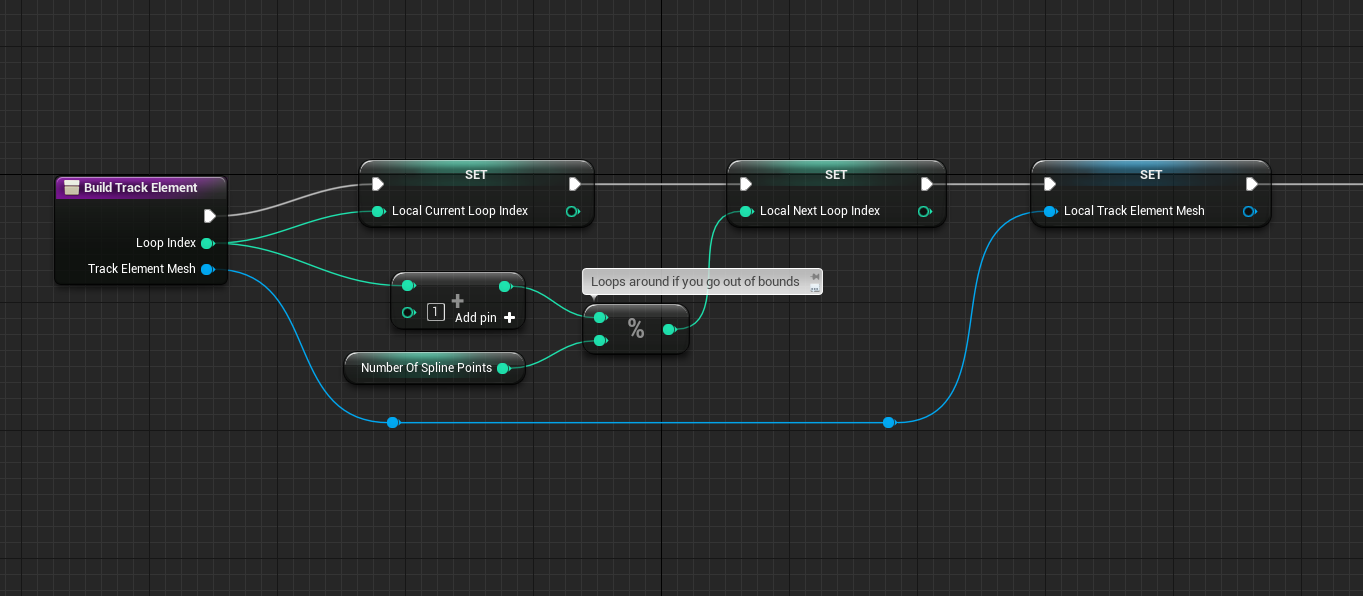
\includegraphics[width=.90\textwidth]{figures/blueprint} @*)
\end{lstlisting}


Students have also suggested the minted package for pretty code listings.  We will consider this in future updates to the coding style at NTNU.

\section{Statistical Analysis}

Many of you will need to use statistics to reject null hypotheses.  There are many statistical packages and ways of analysing data.  Your supervisor should be able to direct you to the type of analytically tool that will allow you to make justifiable claims.

There are some key things to remember.  If you want to make a claim that thing A is better than thing B, then you are rejecting the null hypothesis that they are the same. Equation~\ref{H0mean} states the null hypothesis as the mean of sample 1 ($\mu_1$) is the same as the mean of sample 2 ($\mu_2$). For example if you were measuring height of men and women you would state that the null hypothesis is that men and women are the same height, then you measure 100 men and 100 women and calculate the mean and standard variation of their height. 
\begin{equation} 
\label{H0mean}
    H_0 : \mu_1 = \mu_2
\end{equation}

The t-test can be used to see what the probability $p$ of seeing the values in the sample that you coming from the same actual population. If you have a $p<0.05$ you have a 95\% probability that the samples are actually different.

Thus you set up the evaluation and show that there is a very low probability that the difference you see is caused by sampling error and therefor they are not the same.  The t-test does this for normally distributed scalar values of data. If you are using a Likert Scale then you do not have scalar data, and it may not be normally distributed.

For non-parametric data you need to make a statement about the sampled values~\cite{Kaptein2010}
\begin{equation} 
\label{H0sample}
    H_0 : \phi_1(x) = \phi_2(x)
\end{equation}

There are lots of good sources for understanding statistics for research.  Most of the wikipedia pages are a good entry to the area. For Likert scale analysis there are new tools~\cite{Kaptein2010} which allow for better assessment of the sample sizes we have in most of our Masters thesis projects.

You should also think about learning R the statisical package for doing analysis.  You can download it by searching for "R on windows" or using the link to a windows implementation of R\footnote{\url{https://cran.r-project.org/bin/windows/base/}}


 % could be results
%\chapter{Implementation}
\label{chap:implementation}
When implementing a real time mesh deformation system certain choices must be made.
Firstly one must decide upon the model to use for the mesh deformation itself, i.e. are we algorithmically solving these problems using proper physics, or do we more brute force it through particle simulation. The algorithmic approach using proper physics will usually yield more realistic results, however, they are usually more complicated to implement,
and might not meet the performance requirements of games. The more brute force approaches such as spring-mass spring systems are usually easier to implement,
and gives good enough results.
Following the decision of models we need to decide on an integration scheme, how should we model the changes in acceleration, position, and velocity of our vertices?
Many different integration schemes exits, such as explicit Euler integration, Runge Kutta, or Verlet Intergration, all with different properties and difficulty of implementation.
Following these choices it is possible to start implementing a mesh deformation system.

\todo{Talk about how the deformation is done without mentioning springs first. I.e. you apply force to it.}
\todo{Also mention the importance of damping.}
\todo{Discuss semi-implicit euler integration scheme. Show math and implementation, discuss advantages and disadvantages with it.}
\todo{Motivate that you choose both your "physics model" and your integration scheme}

\section{What is Spring Mass Damping?}
The spring mass damping model is usually presented in a quite intuitive manner.
Each vertex within a mesh is considered a point with its own mass.
Between the vertices are springs which try to hold the whole mesh together.
When no forces are applied to the vertices within the model, the length of the springs are in their desired \rephrase{"resting" state.}
When a forces are applied to the vertices and they start moving, the springs holding the vertices together will become stretched
and will try to get back to their resting state.

\todo{Add image}

\section{What is Semi-Implicit Euler Integration?}
Semi-Implicit Euler integration is perhaps the integration scheme that is easiest to follow, and comes most natural to programmers when they implement
movement in a realtime system for the first time. It is also a scheme used within a lot of physics engines\cite{gafferongames_integration}.
In Semi-Implicit Euler integration we keep the total accumulated force, velocity and position of each game object.
Upon each timestepped update of the system we divide all the force that has been applied to an object by the mass of the object to get the acceleration of the object.
Multiplying this acceleration with the timestep yields the change in velocity of the object, which added on the previous velocity becomes the new velocity.
This new velocity is then multiplied with the timestep and added to the position, reflecting the change in position over time.
The code for this can be seen in listing~\ref{code:semi-implicit_euler}

\begin{figure}
\begin{lstlisting}[label={code:semi-implicit_euler},language=csharp,caption={Semi-Implicit Euler Integration}]
private void Timestep(float deltaTime, GameObject go)
{
    var acceleration = go.force / go.mass;
    go.velocity += acceleration * deltaTime;
    go.position += go.velocity * deltaTime;
}
\end{lstlisting}
\end{figure}

\subsection{Advantages \& Disadvantages}
The largest advantage of the Semi-Implicit Euler integration is its ease of implementation, as well as the generally low computational complexity.
However, it is not entirely stable, meaning that you can get into situations where your numbers start exploding.

\section{What is Verlet Integration?}
Verlet integration 
\subsection{Advantages}
\subsection{Disadvantages}

\section{Implicit Springs - Ball Deformation}
\todo{Add video}
\todo{Add how force is applied, showing the picture from the tutorial}
Jasper Flick\cite{catlike_mesh_deformation} shows an implementation \rephrase{without explicit springs}, following a semi-implicit euler integration scheme.
In this implementation we keep a copy of the initial vertex positions, as well as a collection of the modified vertices.
Additionally, we keep a collection of the velocity of each vertex, which we update each time force is added to a vertex.
The springs come into play when updating the positions of all the vertices based on their velocities.
Each spring within this system is the vector between the initial positions of the vertices in the mesh and their current positions, as seen in figure \ref{fig:catlike_mesh_deformation_springs}.
Upon update of the vertices the force of a spring is applied to the velocity of a vertex in the direction of the spring, moving the vertex back towards its initial position (see listing~\ref{code:catlike_mesh_deformation_update}).

\begin{figure}
%\centering
    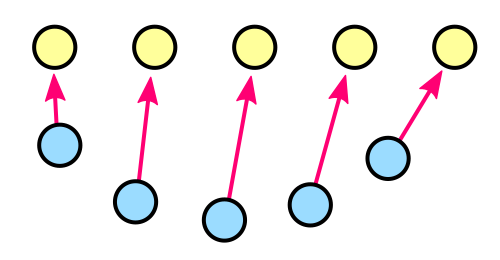
\includegraphics[width=\textwidth]{report/figures/catlike_mesh_deformation_springs.png}
    \caption{Modified vertices(yellow) are pulled towards their original position(blue) by the springs (pink)\cite{catlike_mesh_deformation}}
    \label{fig:catlike_mesh_deformation_springs}
\end{figure}

\begin{figure}
\begin{lstlisting}[label={code:catlike_mesh_deformation_update},language=csharp,caption={Catlike coding mesh deformation vertex update}]
private void UpdateVertex(int i)
{
    Vector3 velocity = mVertexVelocities[i];
    Vector3 spring = mDisplacedVertices[i] - mOriginalVertices[i];
    spring *= UniformScale;
    velocity -= spring * SpringForce * Time.deltaTime;
    velocity *= 1f - Damping * Time.deltaTime;
    mVertexVelocities[i] = velocity;
    mDisplacedVertices[i] += velocity * (Time.deltaTime / UniformScale);
}
\end{lstlisting}
\end{figure}

\subsection{Usage}
As seen from the video, although simple, the implementation provides quite a lot of flexibility, toying with the different variables
can lead to some interesting visual effects.
For example, applying negative force to the sphere can be used to create a visual effect similar to that of a star being swallowed by a black hole.
Applying outward force from the inside of the model can create a relatively convincing effect of something moving around inside the object.
Giving the sphere a high SpringForce will lead to it being harder to deform, and more bouncy when trying to return to its original shape.

\subsection{Limitations}
As previously mentioned the implementation is quite simple, but has some limitations.
As mentioned by Flick\cite{catlike_mesh_deformation} this implementation is not a physics simulation, while the mesh is deformed
the colliders and physical representation of the object stays the same.
Additionally, none of the vertices are connected to each other through springs, and therefore move completely independent from each other.
This means that if we were to for instance pin two of the vertices to their initial position, and then apply force to the mesh
none of the other vertices would respect that two of them was locked in place, leading to less than satisfying results.




\section{Explicit Springs - Cloth Simulation}
\todo{This is a kinematic system, not a dynamic one, so should rename all the springs reference to constraints?}
Cloth simulation is a place where the springs are more apparent than the previous implementation.
The implementation seen in Figure \ref{fig:my_cloth_implementation_springs} shows all the springs needed to create a believable cloth simulation.
The implementation is based on that of Jesper Mosegaard\cite{mosegaards_clothing_simulation}.
Unlike the previous implementation, the springs here are explicit and ensure that vertices are not handled in isolation but rather are affected by the other vertices in the system.
This gives greater control in that it allows you to apply force to a specific vertex and the whole system responds, rather than having to apply the force to all the vertices.

\think{Need to start to segue into the spring types}

\todo{Find the gamasutra article that discussed this}


\begin{figure}
%\centering
%    \caption{\todo{Insert figure}}
    \label{fig:my_cloth_implementation_springs}
\end{figure}


\subsection{Spring Types}
There are three types of springs within this implementation, all serving the same purpose of holding the model together,
but in different ways.

\subsubsection{Structural Springs}
The structural springs are the vertical and horizontal connections between the vertices,
ensure that the model stays in one piece.
However, they alone are not enough, as the model can collapse into itself in a two dimensional space.
\todo{Add small figure showing the structural springs}
\todo{Add small figure showing the model collapsing into itself with just structural springs}

\subsubsection{Shear Springs}
Shear springs fixes the issue mentioned above by a connection between each vertex and their diagonal members.
When the vertices are about to start collapsing in on themselves the shear springs will push them apart again.
\todo{Rewrite this to make it clearer what I mean with 3 dimensional space}
These springs also helps the model to act in a three dimensional space.
Since the vertices no longer can collapse in on themselves they might need to make use of three dimensions to
resolve their collisions.
\todo{Add small figure showing the shear springs, and the model using shear springs}

\subsubsection{Bending Springs}
Technically you only need these two types of springs to create an ok looking cloth simulation,
however a third type of spring called bending springs can be added.
These are connected between each vertex and their second neighbour,
which can help fix cases where the second neighbour of a vertex is unrealistically placed in the system.
This in general leads to the cloth becoming more flat, as extreme differences between the vertices are corrected for
through the second neighbouring vertices.

\todo{Add Drawing}
% This might be what is creating wrinkles?
% Double check that this is actually the case.
% Without
%
% 1 -- 2
%      |
%      3
% With
% ------------|
% 1 -- 2 ---| |
%           3 -
\todo{Add small figure showing the bending springs, and the model using the bending springs}

\subsection{Implementation}
\todo{Go deeper into implementation, the meaning of the constants, showing the code, etc}

\subsection{Usage}
Due to its more sophisticated nature this implementation offers more flexibility than the previous one.
Simulation of entire pieces of clothes like curtains or flags are obvious ways of using this model.
However, it is not a requirement of the model that every vertex in a mesh are simulated and part of the mass spring system, you can also just simulate parts of it.
An example here is if you have a character wearing a dress, you probably do not need that every part of the dress
has realistic cloth physics, it is probably enough that just the bottom of the dress reacts to the environment
to create a believable appearance.
\todo{Add image showing parts of the model being simulated, as I don't think it is entirely clear from the text}

Another use case with this model could be to have cloth that tears at a certain point because it is stretched too much,
or that parts of the cloth is cut off. This should not be too difficult, you would need to remove the springs between
the vertices that have been disconnected from the rest of the model.
Additionally, you would have to ensure that all the cuts were in line with the triangles of the mesh.

\subsection{Issues}
Although there are many advantages of this model, like how it is relatively easy to implement, gives quite good results and cannot "explode", it does suffer from a few issues.
A problem with this implementation is that it can get into unsolvable states.
I.e. when you apply forces to model continously it can get into a situation where it never rests.
Such a situation can be seen in the following video \todo{Add video}.
Here the forces of gravity are continously being applied to the vertices, in the real world the bottom
of this cloth would stop moving after a while. However, in this implementation the cloth never stops moving
because the springs never manage to get into a situation where they all are "satisfied".
The number of times you need to iterate over the constraints to satisfy them is also an issue.
Too few iterations and the cloth will look too elastic, too many iterations and it can seem too hard,
additionally, the more iterations you add, the more processing time is needed, which can become a performance problem.

\subsection{Extensions}
Matthew Fisher\todo{Cite: https://graphics.stanford.edu/~mdfisher/cloth.html} suggests some extensions to the model,
such as quilting.
\todo{Expand on the points Matthew Fisher Brings up}

\todo{Bring up how this model can get into unsolvable states when forces are applied continously}
\todo{Having to iterate over all the springs multiple times isn't optimal}

\todo{Should I also look into the Catlike Coding water deformation thingy, as it is another way of doing mesh deformation}


\todo{The technology ahead, ask if this could be used with tesselation and be done on the GPU?}
\todo{Discuss how mass spring damper model also used for other stuff, such as water simulation. Look at Just Cause water implementation article on gamasutra}

%\chapter{Discussion}
\label{chap:discussion}

The results you have collected and the process you when through to develop the project have been presented earlier.  This Chapter is used to talk about your interpretations of results or the process.  It might be a discussion of the language you used.  A tool that you started to use but then stopped using for some reason.  It could give insight into the evolution of your process.

\todo{ give more examples of discussions}
%\chapter{Conclusion}
\label{chap:conclusion}

This is where you provide an overview of the thesis now that it is finished.  What are the critical things that can be learnt from the thesis for the reader.

This is additional text.

\section{Future Work}
\label{sec:future}
Where would the project go from here.

\todo{again more examples and discussion about what it means to plan}

\todo{there are many more things to say}

\ifthenelse{\boolean{HarvardCitations}}{%
	\bibliographystyle{agsm} % used for Harvard style references. Names - Humanities & Interaction Design
}{%
	\bibliographystyle{ntnuthesis/ntnuthesis} %used for Vancover style references. Numbers - Computer Science & Physics
}

\bibliography{MastersExample}

\appendix
\chapter{Testing Data}
This could be a log of the testing sessions and raw data that is too long for the thesis.
\section{Test Session 1}
\subsection*{Objective}
The Objective of this testing session was to test Hypothesis ....

\subsection*{Participants}
The participants were a convenience sample of students from NTNU. Age range $19-55$ Median age $23$ ...

\subsection{Raw Data}





%\include{inc/timetable}

\end{document}
